\documentclass{beamer} 
% "Beamer" is a word used in Germany to mean video projector. 
%Reference for the ProgressBar Theme 
% http://recherche.noiraudes.net/fr/LaTeX.php
\usetheme{progressbar}

% \usefonttheme{professionalfonts} % using non standard fonts for beamer
\usepackage{iwona}

\usefonttheme{serif} % default family is serif


\graphicspath{{images/}}


\setbeamertemplate{caption}[numbered]
% Beamer Presentation: Figure has no number?
% tex.stackexchange.com/questions/127145/


\usepackage{xmpmulti}
% http://choorucode.com/2010/02/09/how-to-do-image-animation-in-beamer/


\usepackage{animate}
% http://tex.stackexchange.com/questions/129618/

% \usepackage{handoutWithNotes}
% \pgfpagesuselayout{1 on 1 with notes landscape}[a4paper,border shrink=5mm]
% http://www.guidodiepen.nl/2009/07/creating-latex-beamer-handouts-with-notes/comment-page-1/


\usepackage{color} % It may be necessary to set PCTeX or whatever program you are using to output a .pdf instead of a .dvi file in order to see color on your screen.
\usepackage{graphicx} % This package is needed if you wish to include external image files.


\theoremstyle{definition} 
\newtheorem*{dfn}{Definition}               
% See Lesson Three of the LaTeX Manual for more on this kind of "proclamation."


\usepackage{array}
% http://tex.stackexchange.com/questions/118190/update-matrix-entries-in-beamer






\usepackage{color}
% https://www.sharelatex.com/learn/Using_colours_in_LaTeX



% \title{Understanding the Reconstructed State Space Using an IMU}
% \title{Chaos Theory Approach to Human Activity Recognition Using Inertial Sensors}
% \title{Human Acitivity Recogntion Using Chaos Theory}
\title{Chaos Theory Approach to\\ Human Activity Recognition\\ Using Inertial Sensors}
\author{P\'erez-Xochicale Miguel Angel} 
\institute{School of Electronic, Electrical and Computer Engineering\\
University of Birmingham, UK\\
November 2014}
\date{} 
% Remove the % from the previous line and change the date if you want a particular date to be displayed; otherwise, today's date is displayed by default.

\AtBeginSection[]  % The commands within the following {} will be executed at the start of each section.
{
\begin{frame} % Within each "frame" there will be one or more "slides."  
\frametitle{Presentation Outline} % This is the title of the outline.
\tableofcontents[currentsection]  % This will display the table of contents and highlight the current section.
\end{frame}
} % Do not include the preceding set of commands if you prefer not to have a recurring outline displayed during your presentation.




\begin{document}

%+++++++++++++++++++++++++++++++++++++++++++++++++++
\begin{frame} 
\titlepage
\end{frame}
%---------------------------------------------------


\section{Genesis} % Since this is the start of a new section, our recurring outline will appear here.

%+++++++++++++++++++++++++++++++++++++++++++++++++++
\begin{frame}
 \frametitle{Open Challenge @ Mexican's \\Tournament of Robotics 2013}

 \begin{columns}[onlytextwidth]
\begin{column}{0.5\textwidth}
 \begin{figure}
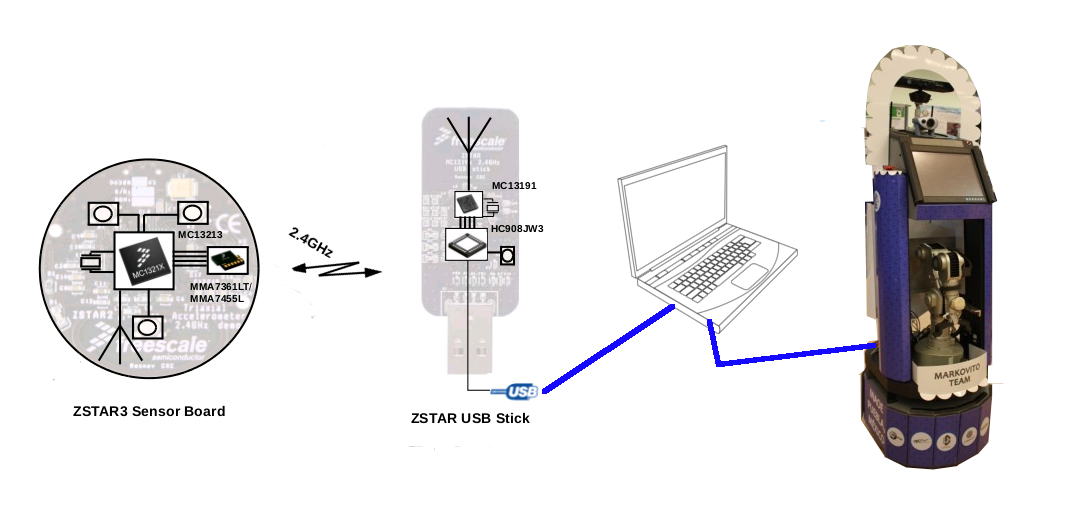
\includegraphics[scale=0.15]{hridd-blockdiagram}
\centering 
\caption{Human-Robot Interface}
\end{figure}
\end{column} 
\begin{column}{0.5\textwidth}
\begin{figure}
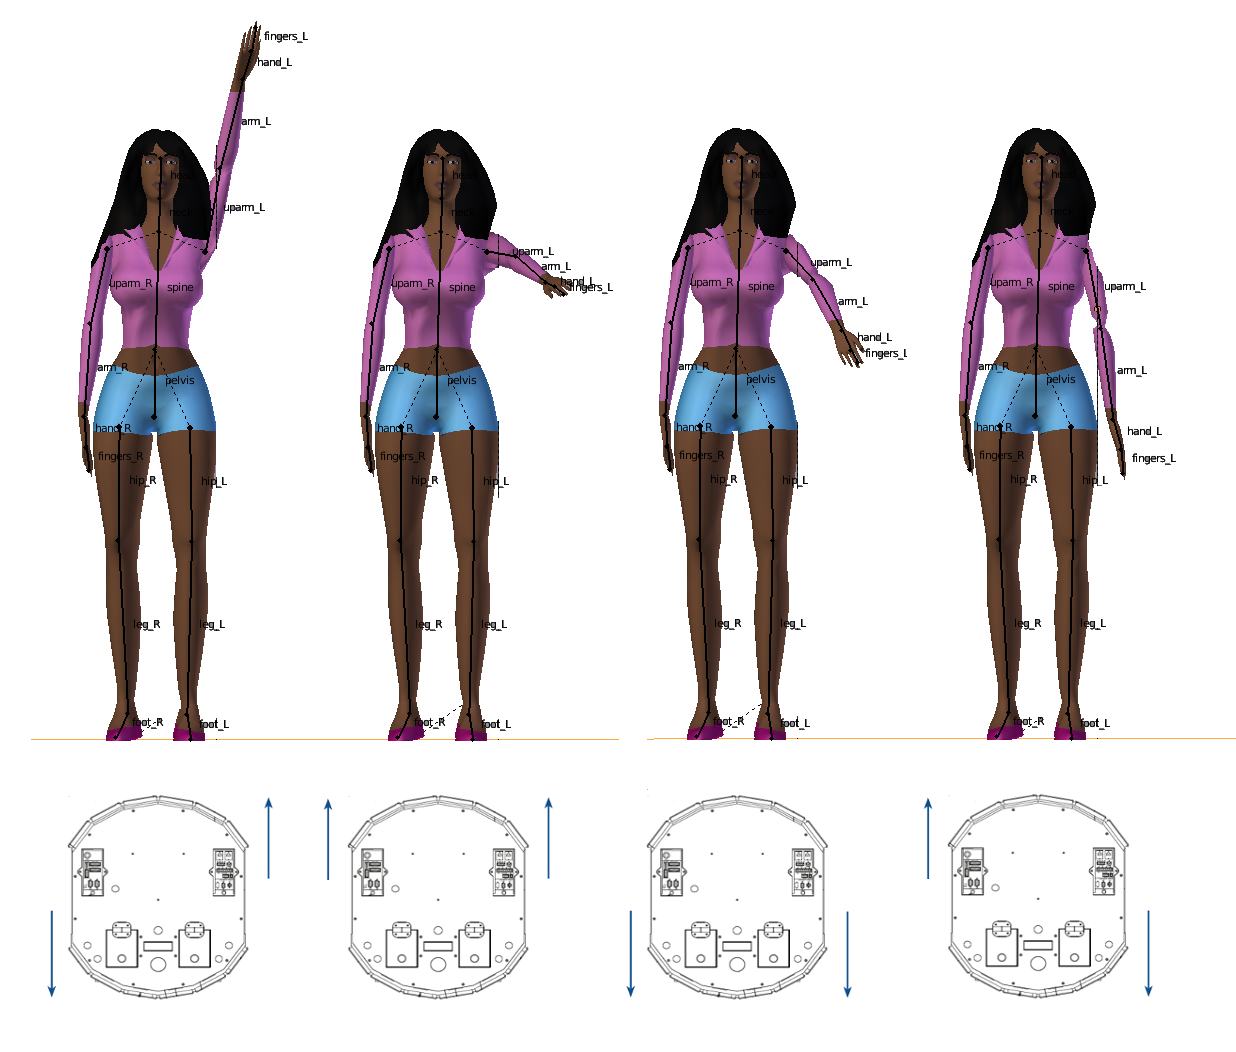
\includegraphics[scale=0.11]{tmr2013demodance}
\centering 
\caption{Human Body Gestures}
\end{figure}
    \end{column}
\end{columns}

\end{frame}
%---------------------------------------------------

\section{Why is Human Activity Recognition (HAR) a challenging task?} % Since this is the start of a new section, our recurring outline will appear here.

% %+++++++++++++++++++++++++++++++++++++++++++++++++++
% \begin{frame}
% 
% \centering
% \fontsize{30pt}{7.2}\selectfont
% Why is Human Activity Recognition (HAR) a challenging task?
% 
% \end{frame}
% %---------------------------------------------------


%+++++++++++++++++++++++++++++++++++++++++++++++++++
\begin{frame}
\frametitle{Challenges in HAR}
\vspace{-0.5cm}
\begin{figure}
 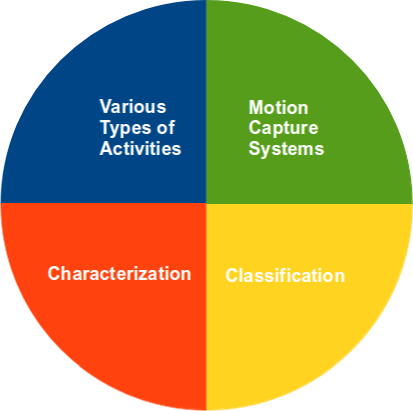
\includegraphics[scale=.4]{why_is_har_a_challenging_task} 
\vspace{-0.6cm}
%  \caption{Reconstructed State Space Via Taken's Theorem}
\end{figure} 
\end{frame}
%---------------------------------------------------






%+++++++++++++++++++++++++++++++++++++++++++++++++++
\begin{frame}
\frametitle{Various Types of Activities}

\begin{table}[h]
\label{t:typesofHAR}
\scriptsize{
\begin{tabular}{|l|l |}
\hline
\textbf{Group }& \textbf{Activities} \\ \hline
Ambulation & Walking, running, sitting, standing still, liying, climbing stairs \\ 
           & descending stairs, riding escalator, and riding elevator. \\ \hline
Transportation & Riding a bus, cycling and driving. \\ \hline
Daily activities & Eating, drinking, working at the PC, watching TV,\\ 
              & reading, brushing teeth, stretching, scrubbing, and vacuumming. \\ \hline
Exercise & Rowing, lifting weights, spinning, Nordic walking \\ 
       & and doing push ups. \\ \hline
Military & Crawling, kneeling, situation assessment and  \\ 
          & openning a door. \\ \hline
Upper body & Chewing, speaking, swallwing, sighing, and moving the head\\ \hline  
Others & Dancing different styles of music: latin, waltz, salsa, etc. \\ \hline  
\end{tabular}}
\caption{Types of activities recognized by Human Activity Recognition
Systems}
\end{table}

\end{frame}
%---------------------------------------------------



%+++++++++++++++++++++++++++++++++++++++++++++++++++
\begin{bibunit}[apalike]
\begin{frame}
\frametitle{Signal Characterization}

\begin{table}[h]
 \label{t:typesofHAR}
\scriptsize{
\begin{tabular}{|l|l |}
\hline
\textbf{Group}& \textbf{Methods} \\ \hline
Time domain & Mean, standard deviation, variance, interquartile range,\\
        & mean absolute deviation, correlation between axes,\\
        & entropy, and kurtosis. \\ \hline  
Frequency domain & Fourier Transform, and Discrete Cosine Transform \\ \hline  
Others & Reconstructed State Space, Principal Component Analysis, \\
      & Linear Discriminant Analysis, Autoregresive Model, \\
      & and HAAR filters.\\ \hline
\end{tabular}}
\caption{Featured Extraction Methods\cite{Lara2013}.}
\end{table}
\biblio{refslides}
\end{frame}
\end{bibunit}
%---------------------------------------------------



%+++++++++++++++++++++++++++++++++++++++++++++++++++
\begin{frame}
\frametitle{Classification}

\begin{table}[h]
\label{t:typesofHAR}
\scriptsize{
\begin{tabular}{|l|l |}
\hline
\textbf{Group }& \textbf{Classifiers} \\ \hline
Decision tree & C4.5 and ID3   \\ \hline  
Instance Based & $k$-nearest neighbors \\ \hline  
Neural Networks & Multilayer Perceptron \\ \hline  
Domain transform & Support Vector Machines \\ \hline  
Fuzzy Logic & Fuzzy Basis Function and Fuzzy Interference System \\ \hline  
Regression methods & MLR, ALR \\ \hline  
Markov models & Hidden Markov Models and Conditional Random Fields \\ \hline  
Classifier ensembles & Boosting and Bagging  \\ \hline  
\end{tabular}}
\caption{Classification Algorithms \cite{Lara2013}.}
\end{table}
\end{frame}
%---------------------------------------------------



%+++++++++++++++++++++++++++++++++++++++++++++++++++
\begin{frame}
\frametitle{Motion Capture Systems}

\begin{columns}[onlytextwidth]
\begin{column}{0.5\textwidth}
\begin{itemize}
 \item Vision-based,
 \item Floor-sensor based, 
 \item Intertial-sensor based:
 \begin{itemize}
  \item Human Body-sensed
  \item Foot-sensed
 \end{itemize}
\end{itemize}
\end{column} 
\begin{column}{0.5\textwidth}
\begin{figure}
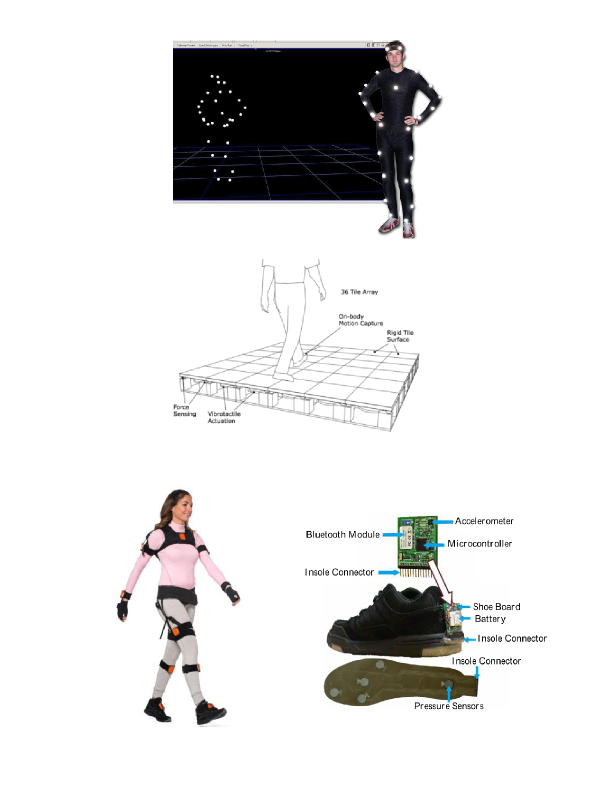
\includegraphics[scale=0.25]{motioncapturesystems}
\centering 
\caption{Motion Capture Systems}
\end{figure}
    \end{column}
\end{columns}
\end{frame}
%---------------------------------------------------



\section{Dynamical System Characterization}


%+++++++++++++++++++++++++++++++++++++++++++++++++++
\begin{frame}
\frametitle{The Human Body as a Complex \\ Dynamical System}
Human Body Movement is the result of a complex dynamical system
 that include:  
\begin{columns}[onlytextwidth]
\begin{column}{0.5\textwidth}
\begin{itemize}
 \item Muscular system,
 \item Cardiovascular system,
 \item Skeletal system, and
 \item Nervous system.
\end{itemize}
\end{column} 
\begin{column}{0.5\textwidth}
\begin{figure}
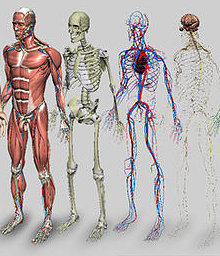
\includegraphics[scale=0.4]{humanbodysystems}
\centering 
\caption{Human Body Systems}
\end{figure}
    \end{column}
\end{columns}

\end{frame}
%---------------------------------------------------


%+++++++++++++++++++++++++++++++++++++++++++++++++++
\begin{frame}
\frametitle{Nonlinear Dynamics in the \\ Human Body}

\begin{figure}
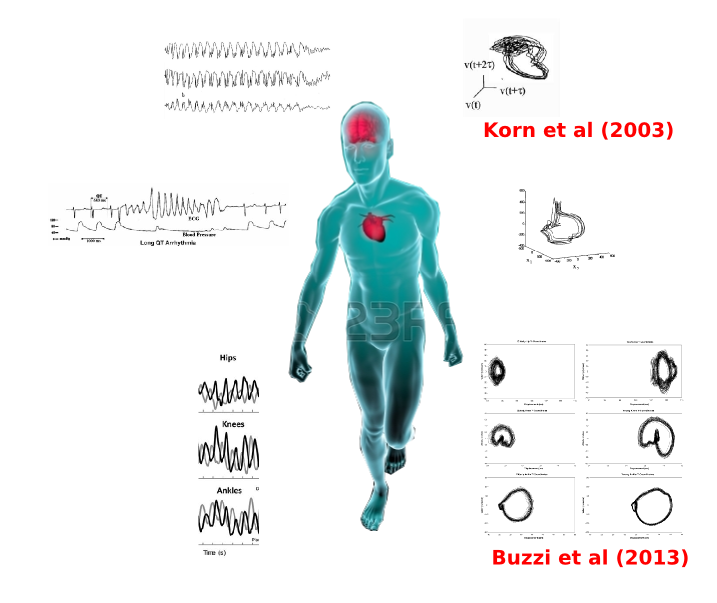
\includegraphics[scale=.3]{timeserieshumanbody}
\centering 
\caption{Some Captured Time-Series from the Human Body}
\end{figure}
\end{frame}
%---------------------------------------------------


%+++++++++++++++++++++++++++++++++++++++++++++++++++
\begin{bibunit}[apalike]
\begin{frame}
\frametitle{Time-Delay Embedding in HAR}

\cite{Jordan2010} and \cite{Sama2013} have proposed the use of 
Taken's Theorem so as to indenfity primitive human activities such as 
walking, cycling, and running. However, little has been done regarding 
the identification of complex activities that, for example, involve dance.

    \vfill
    \biblio{refslides}
\end{frame}
\end{bibunit}
%---------------------------------------------------




\section{What Is Time-Delay Reconstruction?}


%+++++++++++++++++++++++++++++++++++++++++++++++++++
\begin{frame}
\frametitle{Lorenz System}
  
 \begin{columns}[onlytextwidth]
   \begin{column}{0.3\textwidth}
\begin{eqnarray*} 
 \frac{dx}{dt} &=&\sigma (x-y), \\
 \frac{dx}{dt} &=&x (\rho -z) - y, \\ 
 \frac{dx}{dt} &=&xy - \beta z.
\end{eqnarray*}
\end{column} 
 
 \begin{column}{0.63\textwidth}
      \begin{figure}
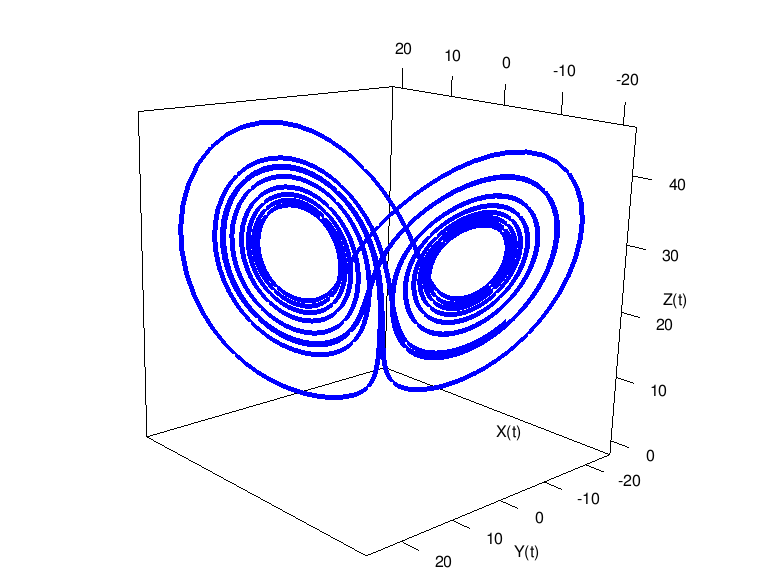
\includegraphics[scale=.25]{lorenzattractor}
 \caption{$\sigma=10$, $\rho=28$ and $\beta=3/8$}
      \end{figure}
    \end{column}
 \end{columns}
\end{frame}
%---------------------------------------------------



%+++++++++++++++++++++++++++++++++++++++++++++++++++
\begin{frame}
\frametitle{Time-Delay Reconstruction}
\vspace{-0.5cm}
\begin{figure}
 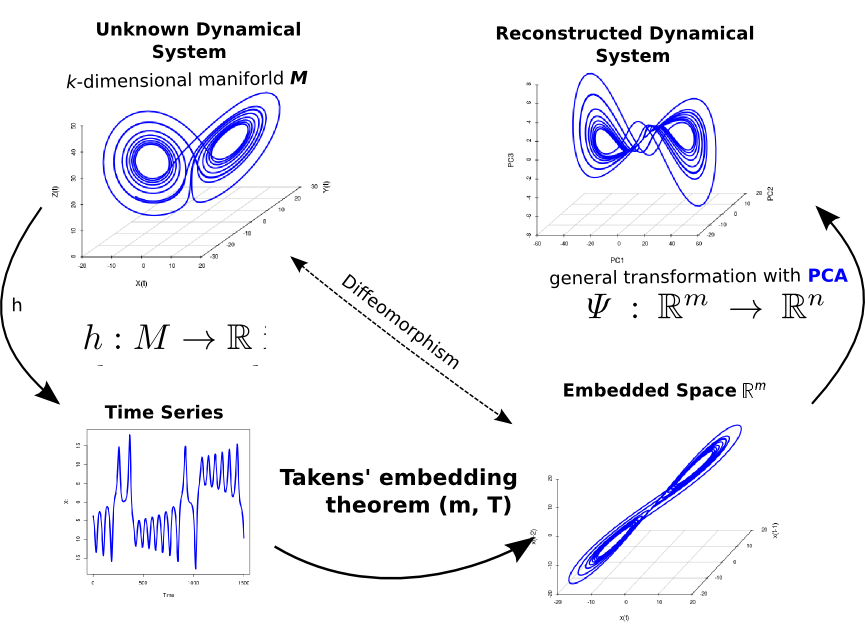
\includegraphics[scale=.4]{takens_theorem_v2} 
\vspace{-0.6cm}
 \caption{Reconstructed State Space Via Taken's Theorem}
\end{figure} 
\end{frame}
%---------------------------------------------------






%+++++++++++++++++++++++++++++++++++++++++++++++++++
\begin{frame}
\frametitle{Takens' Theorem (1981)}


According to Takens' Theorem, the reconstructed state space
in  \textbf{$m$ embedding dimension} with  \textbf{ $\tau$ embedding delay}
of the original system is given by the delay coordinate (DC) vector

\begin{eqnarray*} 
\overline{x(t)} = (x(t), x(t - \tau), x(t-2\tau), ... , x (t-(m-1)\tau).
\end{eqnarray*}
 
Takens' Theorem, also knows as time-delay embeddings method, states
that for a large enough $m$ to unfold the attractor and $\tau > 0$ 
chosen to maximize the information
content of $x(t)$, this method provides a 
one-to-one reconstruction
of the true dimension $k$ system ($\mathbb{R}^k$).


% state space 

% Takens' Theorem, also knows as time-delay embeddings method, is useful 
% when one does not have access to the the true dimension $k$
% state space $\mathbb{R}^k$. Henceforth, it has been demostrated
% that one can obtain a manifold in $\mathbb{R}^m$ that is one-to-one
% and preserves local differential structure.


% One can represent a multidimensional phase
% space of by using the Taken's Theorem.
% 
% Let $o_t$ be the time series, 
% The time-delay reconstruction in $m$ dimensions with the time delay $\tau$
% 
% \begin{eqnarray*} 
% E_t : \mathbb{R}^k \rightarrow \mathbb{R}^m 
% \end{eqnarray*}

% It's natural to think that if $g'(c)>0$ then $g$ must be ``increasing at $x=c$.'' 
% \pause But what does ``increasing at $x=c$'' really mean?
% \pause 
% Taken's Method

% \begin{dfn} % We created the proclamation dfn near the start of the document.
% A function $g$ is \emph{increasing at $x=c$} if there 
% is an open interval $I=(c-\delta,c+\delta)$ such that \pause if $x_1, x_2\in I$, \pause then $x_1<x_2\Rightarrow \pause g(x_1)<g(x_2)$.
% \end{dfn}
\end{frame}
%---------------------------------------------------


% 
% \begin{frame}{Row-echelon form}
%   Reduce the following matrix to row-echelon form.
%   \[ 
%   \begin{bmatrix}
%     \overline{x(1)} \\
%     \overline{x(2)} \\
%     \overline{x(3)} \\
%     \overline{x(4)} \\
%     \overline{x(5)}
%   \end{bmatrix}
%   \onslide<2->
%   \to
%     \begin{bmatrix}
%     1 & 3 & 5 \\
%     2 & 4 & 6 \\
%     3 & 5 & 7 \\
%     4 & 6 & 8 \\
%     5 & 7 & 9 
%   \end{bmatrix}
%   \]
% \end{frame}



%+++++++++++++++++++++++++++++++++++++++++++++++++++
\begin{frame}
\frametitle{Time-Dalay Embedding Example}

With time signal $x(i) = \{ 1,2,3,4,5,6,7,8,9 \} $, we let $m=3$, $\tau=2$, and $N=9$.


\begin{eqnarray*} % As usual, the asterisk suppresses the numbering of each line in the array.
\overline{x(1)} &=& [ 1, \quad 3, \quad 5] \\
\overline{x(2)} &=& [ 2, \quad 4, \quad 6] \\
\overline{x(3)} &=& [ 3, \quad 5, \quad 7] \\
\overline{x(4)} &=& [ 4, \quad 6, \quad 8] \\
\overline{x(5)} &=& [ 5, \quad 7, \quad 9] 
\end{eqnarray*}

Let $M = N-(m-1)\tau$. The reconstructed state space consist of
a $m \times M$ matrix.
% whose $i$th colum is 
% $\overline{x(t)} = (x(t), x(t - \tau), x(t-2\tau), ... , x (t-(m-1)\tau).$


\end{frame}
%---------------------------------------------------





% 
% %+++++++++++++++++++++++++++++++++++++++++++++++++++
% \begin{frame}
% \frametitle{Time-Delay Embedding Example }
% 
% \begin{figure}
%  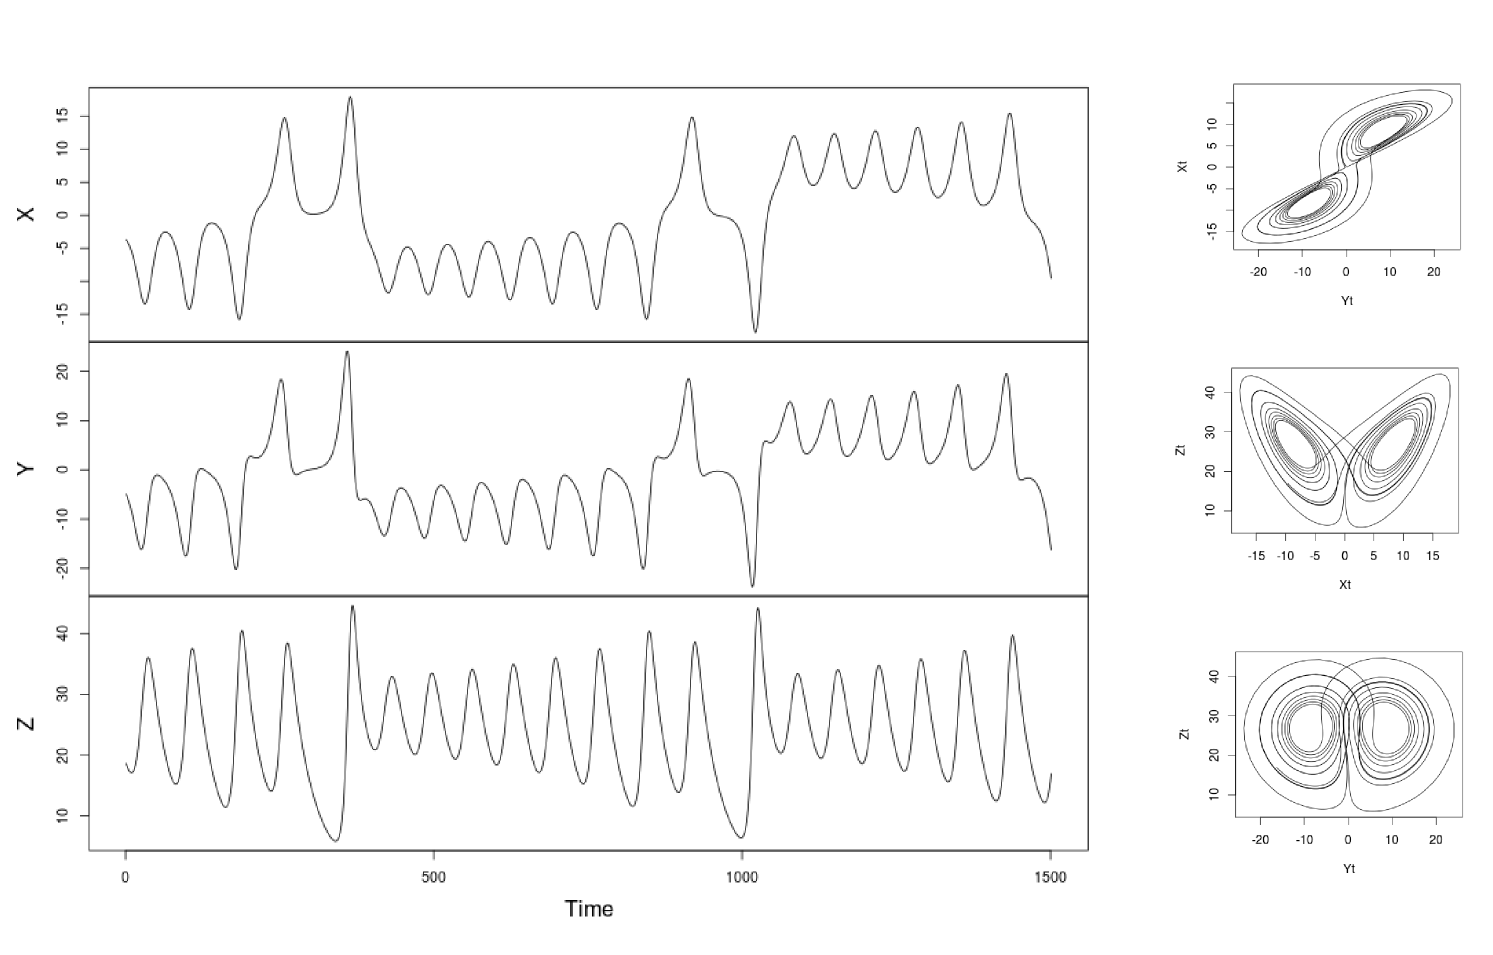
\includegraphics[scale=.2]{timeseries_2dmanifolds} \\
% \caption{Time series of the Lorenz System and 2D manifolds}
% \end{figure} 
%  
% \end{frame}
% 
% 
% 
% % %+++++++++++++++++++++++++++++++++++++++++++++++++++
% % %%%%%%%%%%%%%%%
% % %%ANIMATION in evince
% % \begin{frame}
% % \frametitle{Time-Delay Embedding Example}
% %  \begin{columns}[onlytextwidth]
% %    \begin{column}{0.5\textwidth}
% % \begin{figure}
% % 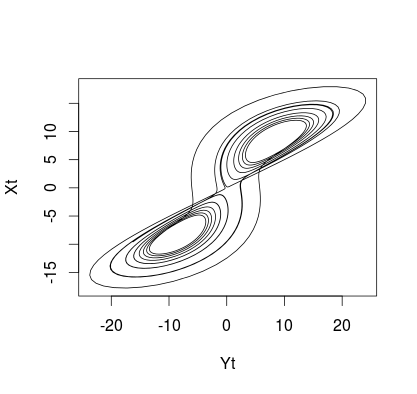
\includegraphics[scale=.3]{XY} 
% % \caption{Original Manifold}
% % \end{figure} 
% % \end{column} 
% %  
% %  \begin{column}{0.5\textwidth}
% % 
% % \begin{figure}
% % % \multiinclude[format=png,graphics={scale=0.3}]{images_frames_for_TAU/manifold_d3_t} 
% % 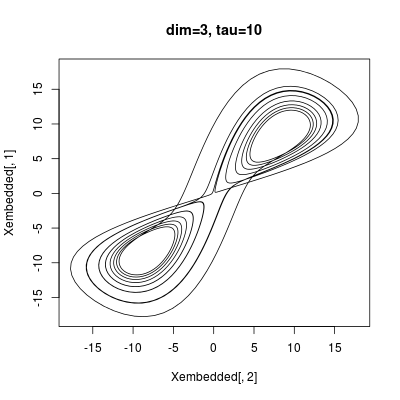
\includegraphics[scale=0.3]{images_frames_for_TAU/manifold_d3_t-10}
% % \caption{Reconstructed Manifold}
% % \end{figure}
% %  \end{column}
% %  \end{columns}
% % \end{frame}
% 
% 
% % %%%%%%%%%%%%%%%
% % %%ANIMATION 2 in adobe acrobat
% % \begin{frame}
% % \frametitle{Time Delay Embedding}
% % 
% %  \begin{columns}[onlytextwidth]
% %    \begin{column}{0.5\textwidth}
% % \begin{figure}
% %  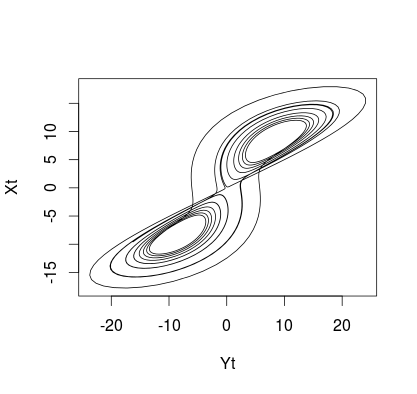
\includegraphics[scale=.3]{XY} 
% % \caption{Time series and 2D manifolds}
% % \end{figure} 
% % \end{column} 
% % 
% %  \begin{column}{0.5\textwidth}
% %   \begin{figure}
% % \animategraphics[autoplay, width=0.7\textwidth]{5}{manifold_d3_tn/manifold_d3_t-}{0}{20}
% % \caption{Time series and 2D manifolds}
% % \end{figure}
% % % \animategraphics[<options>]{<frames per second>}{<name without extension>}{<first frame>}{<last frame>}
% % %it only works with adobe acrobat
% %  \end{column}
% % \end{columns}
% % \end{frame}
% 
% 
%---------------------------------------------------


%+++++++++++++++++++++++++++++++++++++++++++++++++++
\begin{bibunit}[apalike]
\begin{frame}
\frametitle{Optimal embedding parameters}

\cite{Cao1997} proposed a method
to determine the optimal embedding dimmension
from time-series based on Taken's theorem.

\begin{figure}
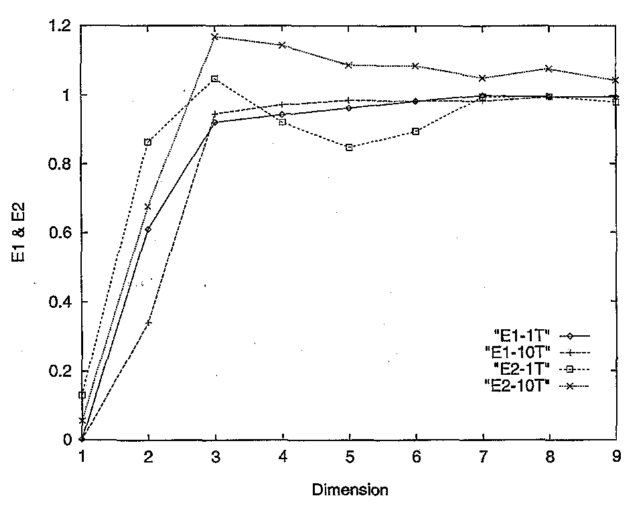
\includegraphics[scale=0.15]{e1e2cao1997}
\caption{The values E1 and E2 for the data from chaotic Lorenz attractor}
% \cite{Li2005}, \cite{Fraser1986}
% }
\end{figure}
%   \vfill
    \biblio{refslides}
\end{frame}
\end{bibunit}
%---------------------------------------------------





%+++++++++++++++++++++++++++++++++++++++++++++++++++
\begin{bibunit}[apalike]
\begin{frame}
\frametitle{Time-Delay Embedding in HAR}

\cite{Jordan2010} and \cite{Sama2013} have proposed the use Taken's Theorems
so as to indenfity primitive human activities such as walking, cycling, and 
running. However, little has been done regarding the identification of
complex activities that, for example, involve dance.

    \vfill
    \biblio{refslides}
\end{frame}
\end{bibunit}
%---------------------------------------------------



\section{Experimentation}

%+++++++++++++++++++++++++++++++++++++++++++++++++++
\begin{frame}
\frametitle{Procedure}

\begin{figure}
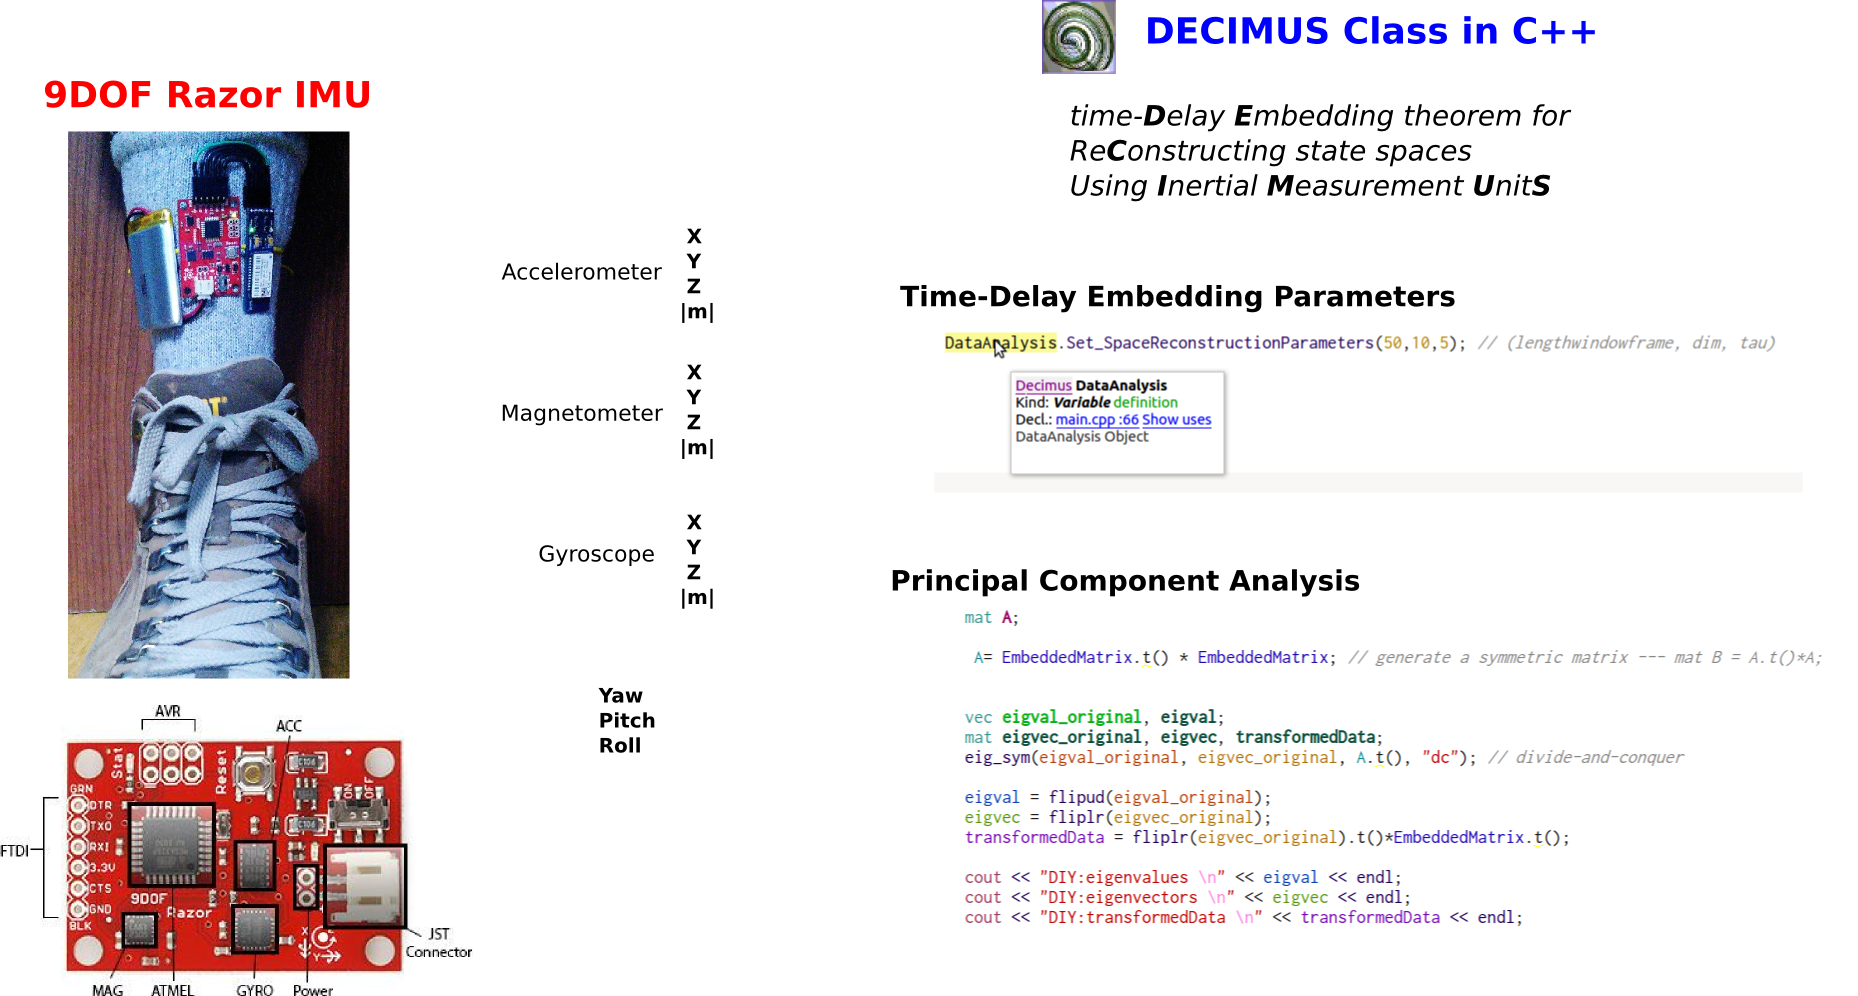
\includegraphics[scale=0.2]{procedure}
\caption{IMU, Axes and C++ Class}
\end{figure}  
\end{frame}


%+++++++++++++++++++++++++++++++++++++++++++++++++++
\begin{frame}
\frametitle{Experiments}

\vspace{-5mm}
\begin{figure}
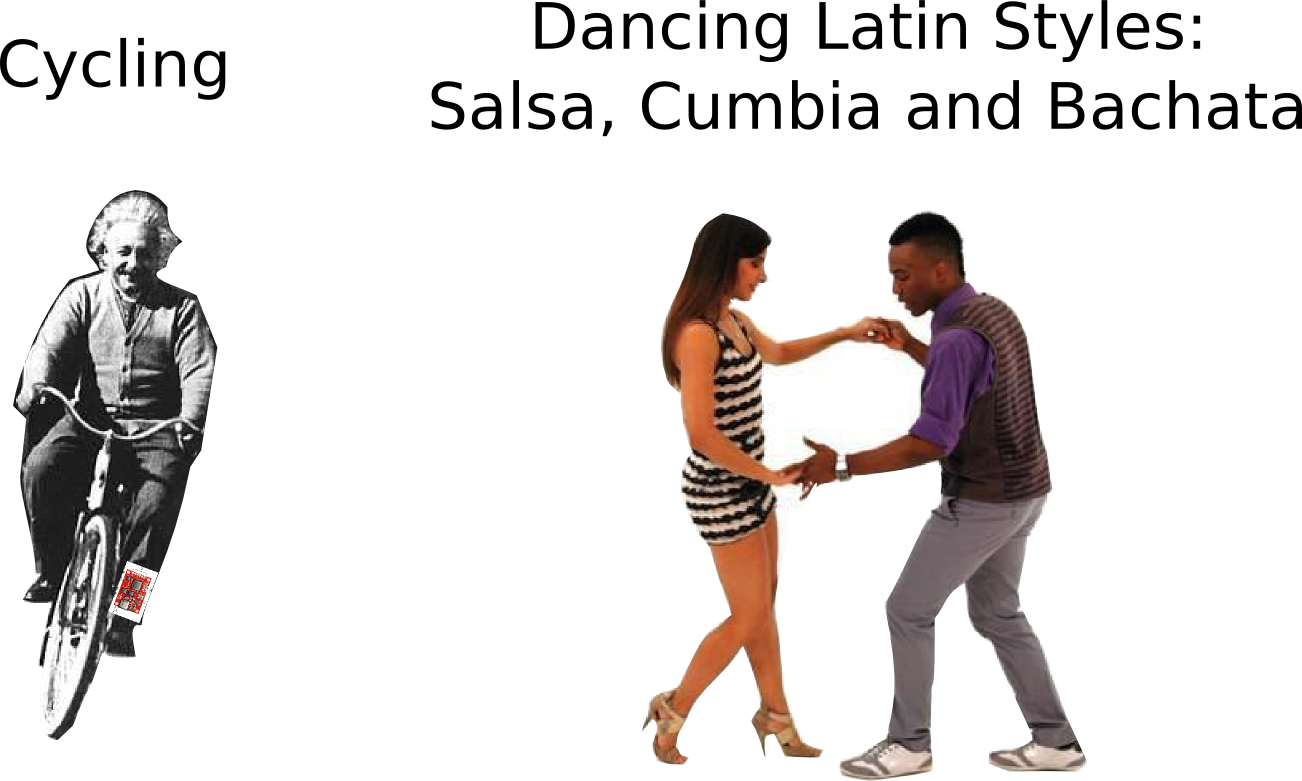
\includegraphics[scale=0.23]{humanbodyactivities}
\vspace{-3mm}
\caption{Human Body Activities}
\end{figure}  
\end{frame}
%---------------------------------------------------




%+++++++++++++++++++++++++++++++++++++++++++++++++++
\begin{frame}
% \frametitle{Cycling}

\vspace{-5mm}
\begin{figure}
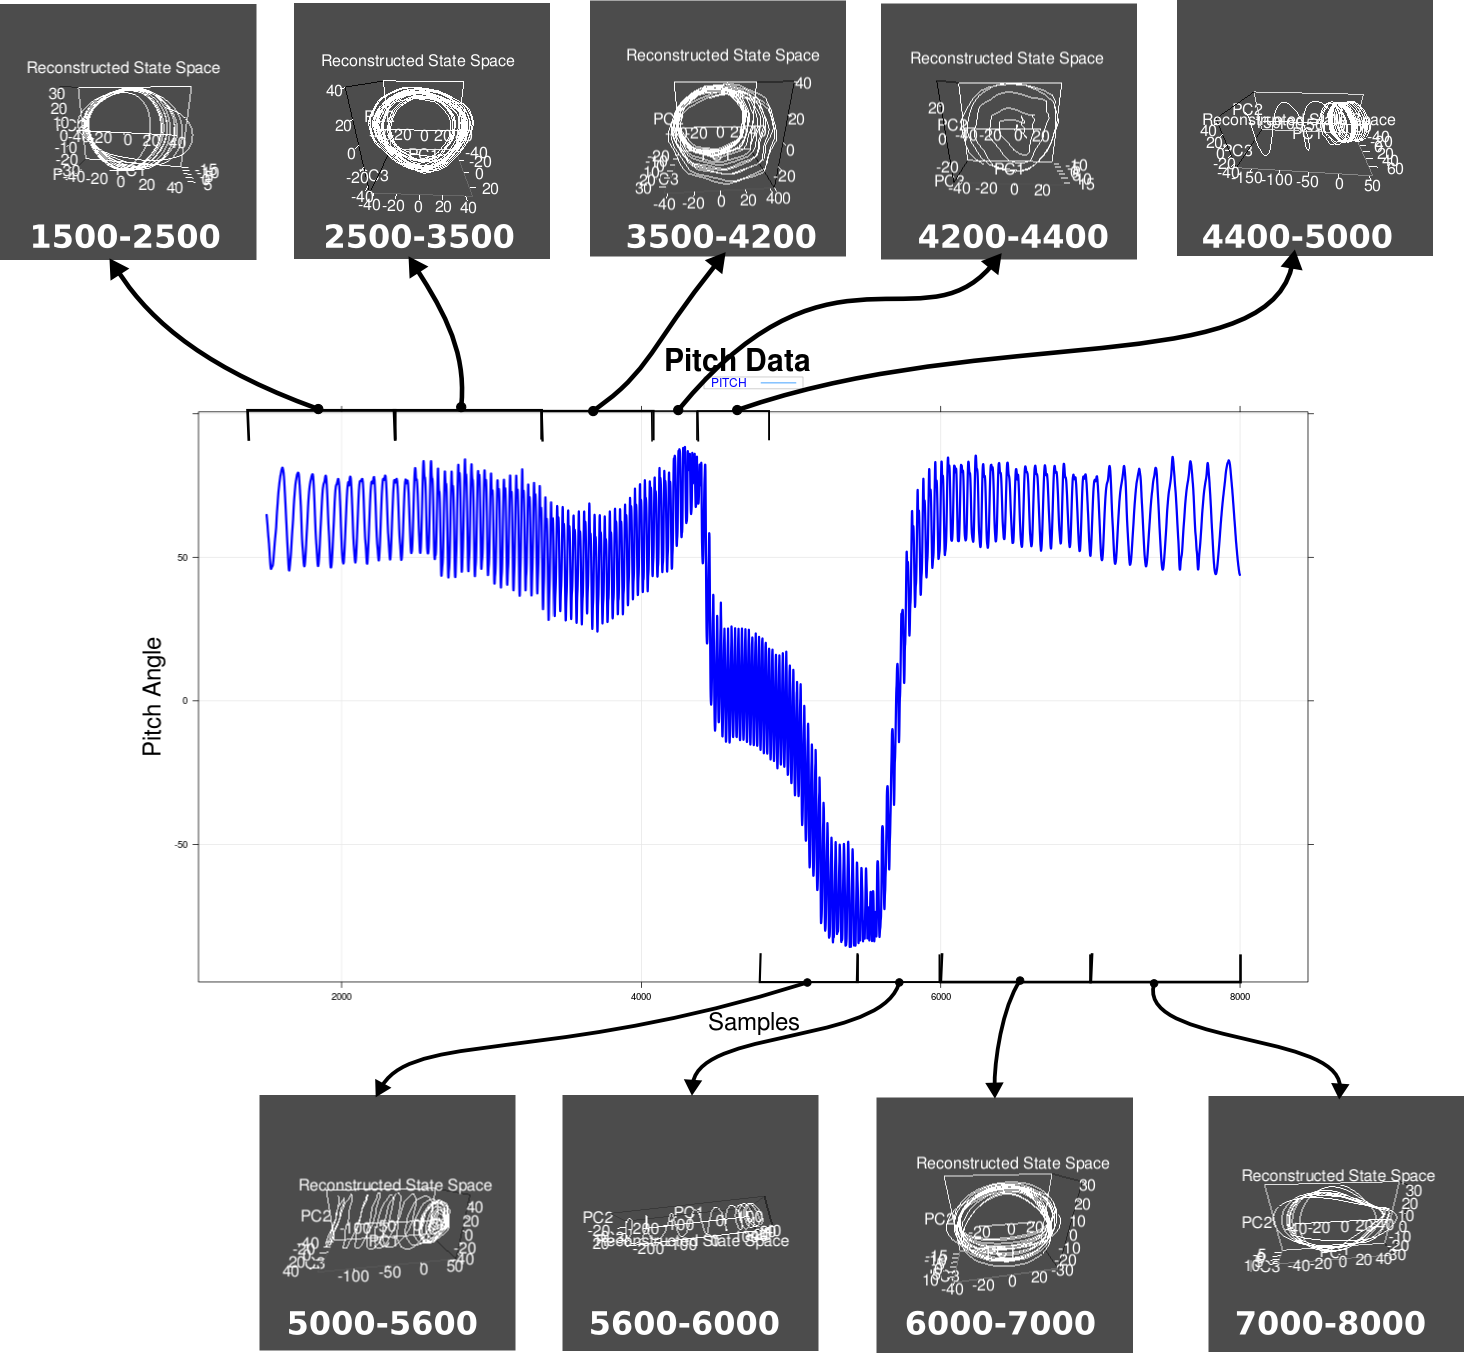
\includegraphics[scale=0.22]{cycling_rss}
\vspace{-3mm}
\caption{3D Reconstructed State Spaces ($m=9, \tau=4$) for pitch angle data 
from cylcling activity}
\end{figure}  
\end{frame}
%---------------------------------------------------





%+++++++++++++++++++++++++++++++++++++++++++++++++++
\begin{frame}
\frametitle{Basic Dance Foot Patterns}

\begin{figure}
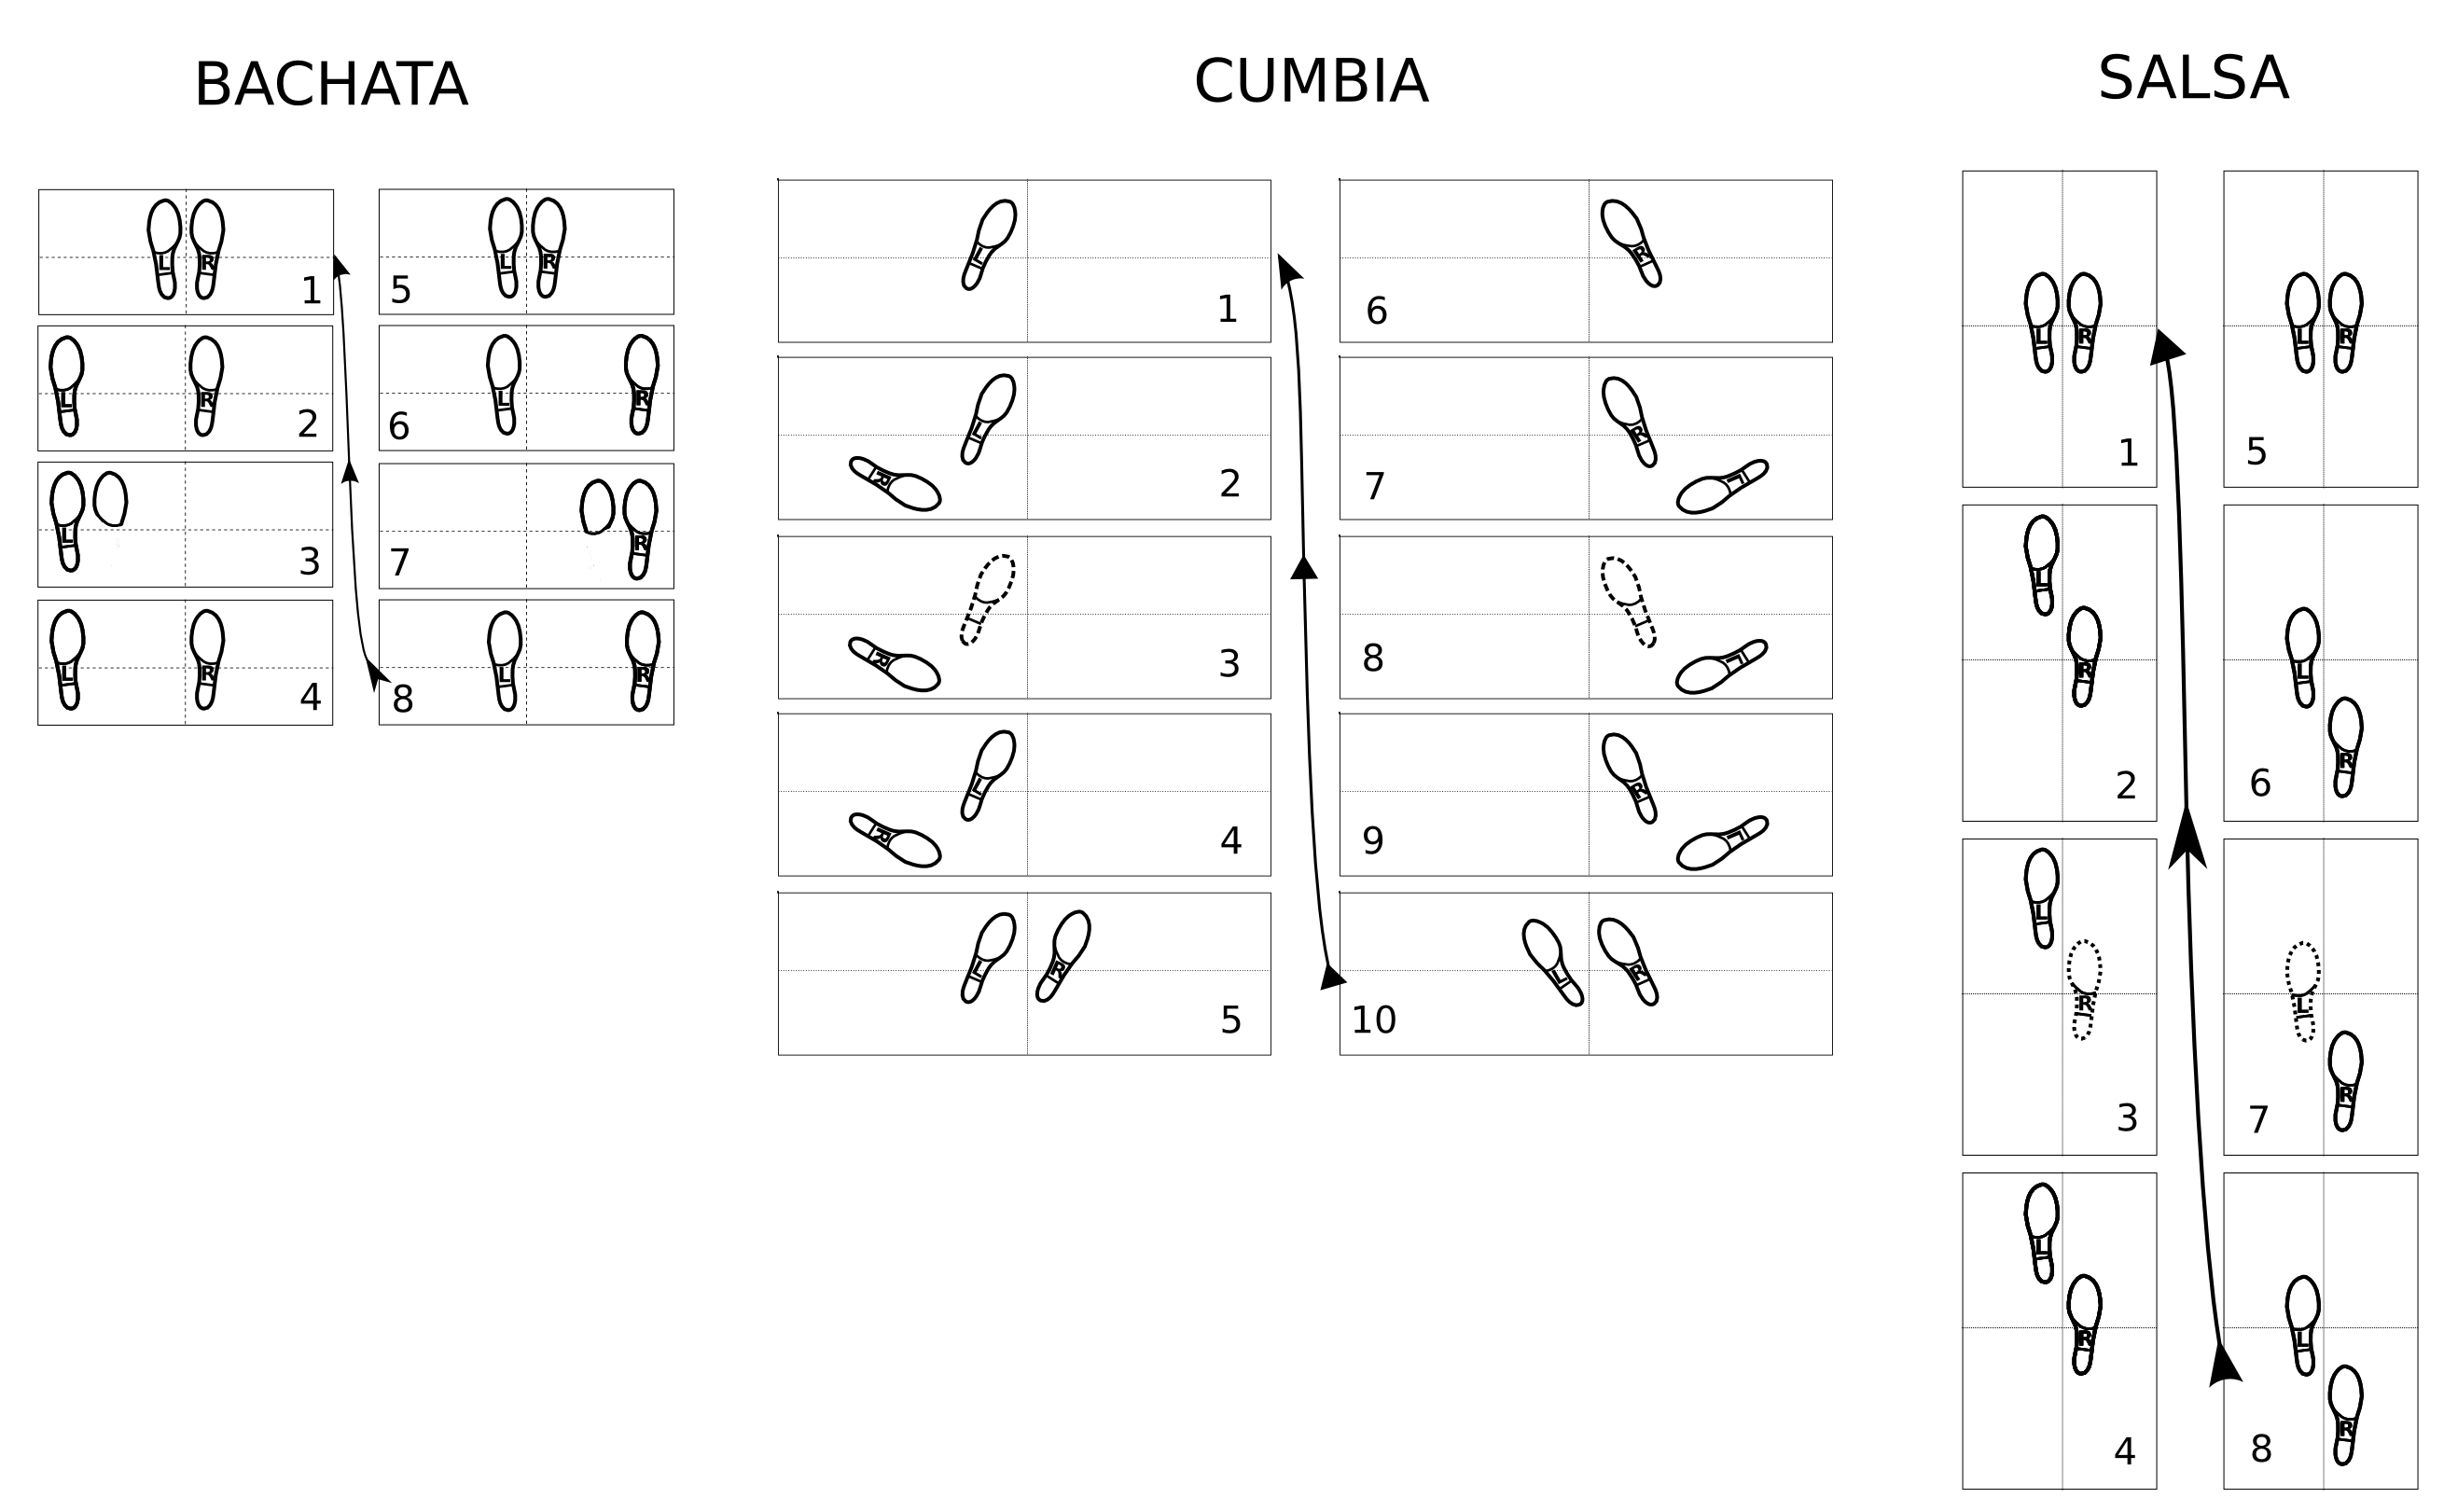
\includegraphics[scale=0.13]{basicdancefootpatterns}
\caption{Latin Dance Foot Patterns}
\end{figure}  
\end{frame}
%---------------------------------------------------






%+++++++++++++++++++++++++++++++++++++++++++++++++++
\begin{bibunit}[apalike]
\begin{frame}
\frametitle{Optimal embedding parameters}

Using the method proposed by \cite{Cao1997}, it has been obtained
the values of E1 and E2 to determine the optimal embedding dimmension
with $\tau=5$ from pitch data.

\begin{figure}
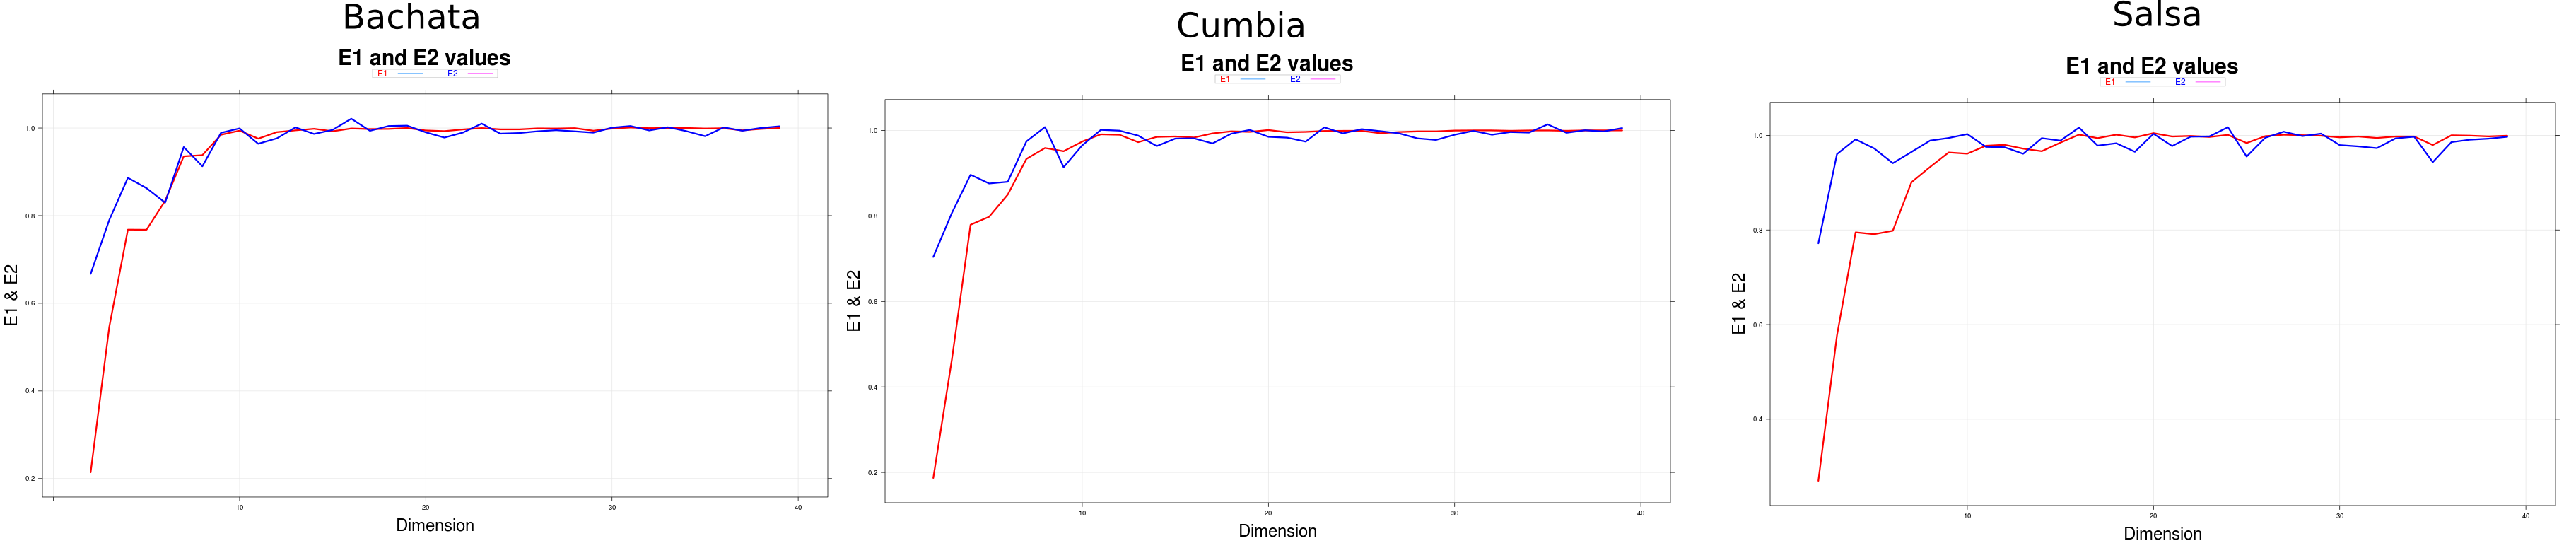
\includegraphics[scale=0.1]{e1e2_bachata_cumbia_salsa}
\caption{The values E1 and E2 for the data from latin dacen foot patterns}
% \cite{Li2005}, \cite{Fraser1986}
% }
\end{figure}
%   \vfill
%     \biblio{refslides}
\end{frame}
\end{bibunit}
%---------------------------------------------------





%+++++++++++++++++++++++++++++++++++++++++++++++++++
\begin{frame}
\frametitle{Reconstructed State Spaces}

\begin{figure}
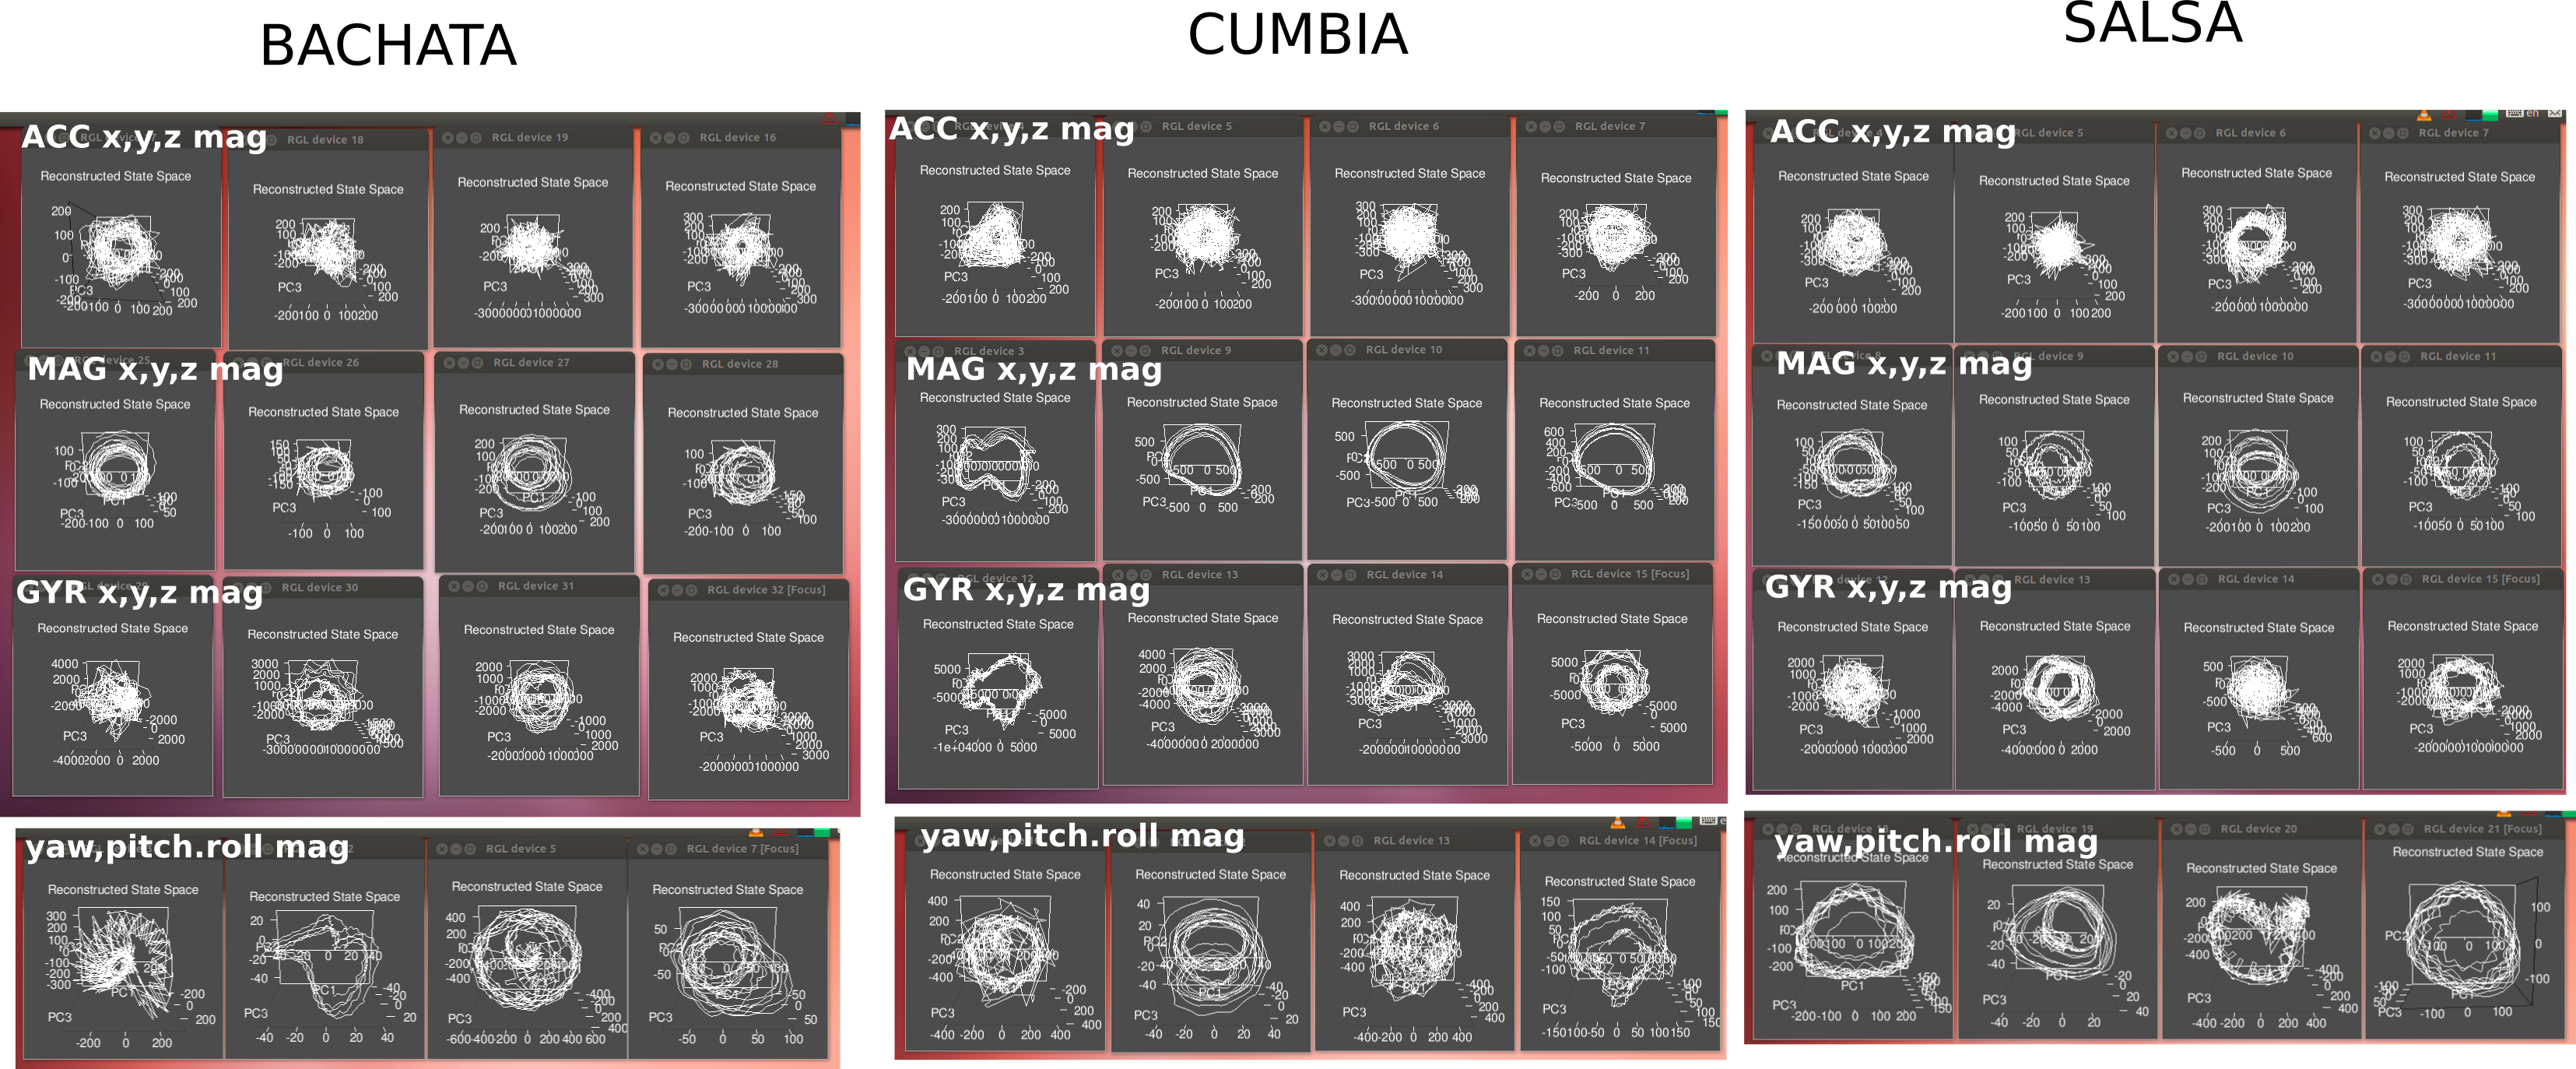
\includegraphics[scale=0.122]{bachata_cumbia_salsa_AccMagGyrYawPitchRoll}
\caption{3D Reconstructed State Space with $m=20$ and $\tau=5$ for a WF=1000.}
\end{figure}  
\end{frame}
%---------------------------------------------------





%+++++++++++++++++++++++++++++++++++++++++++++++++++
\begin{frame}
\frametitle{Pitch Angle Time Series for Bachata}

\begin{figure}
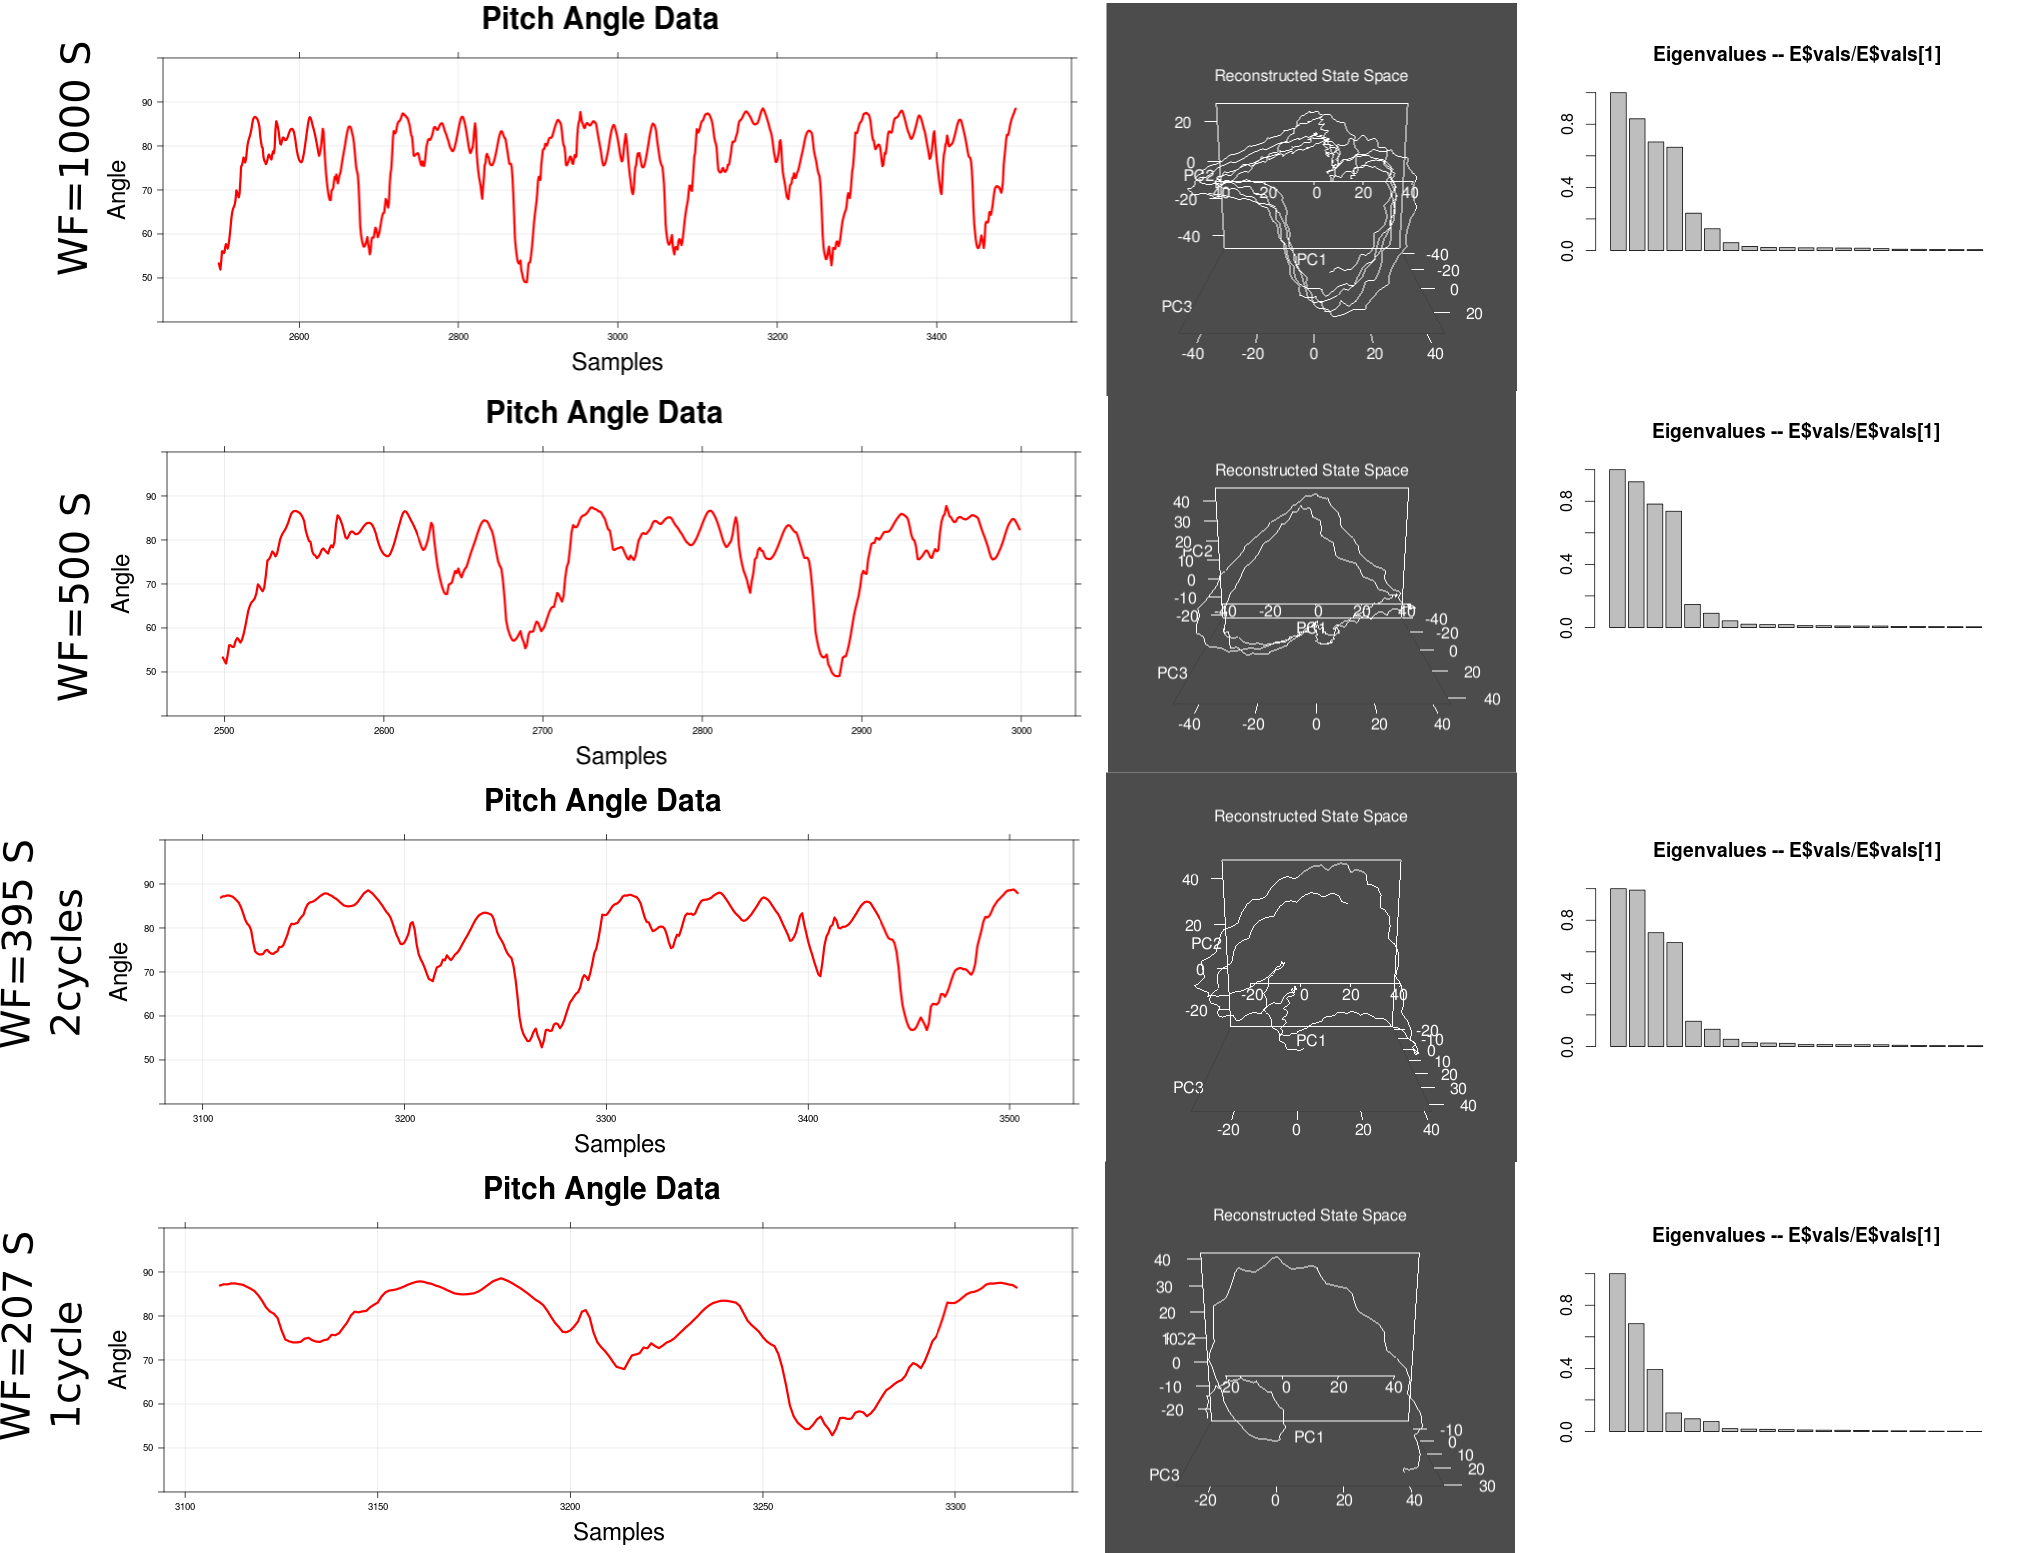
\includegraphics[scale=0.129]{bachata}
\caption{3D Reconstructed State Space and Eigenvalues}
\end{figure}  
\end{frame}
%---------------------------------------------------


%+++++++++++++++++++++++++++++++++++++++++++++++++++
\begin{frame}
\frametitle{Pitch Angle Time Series for Cumbia}

\begin{figure}
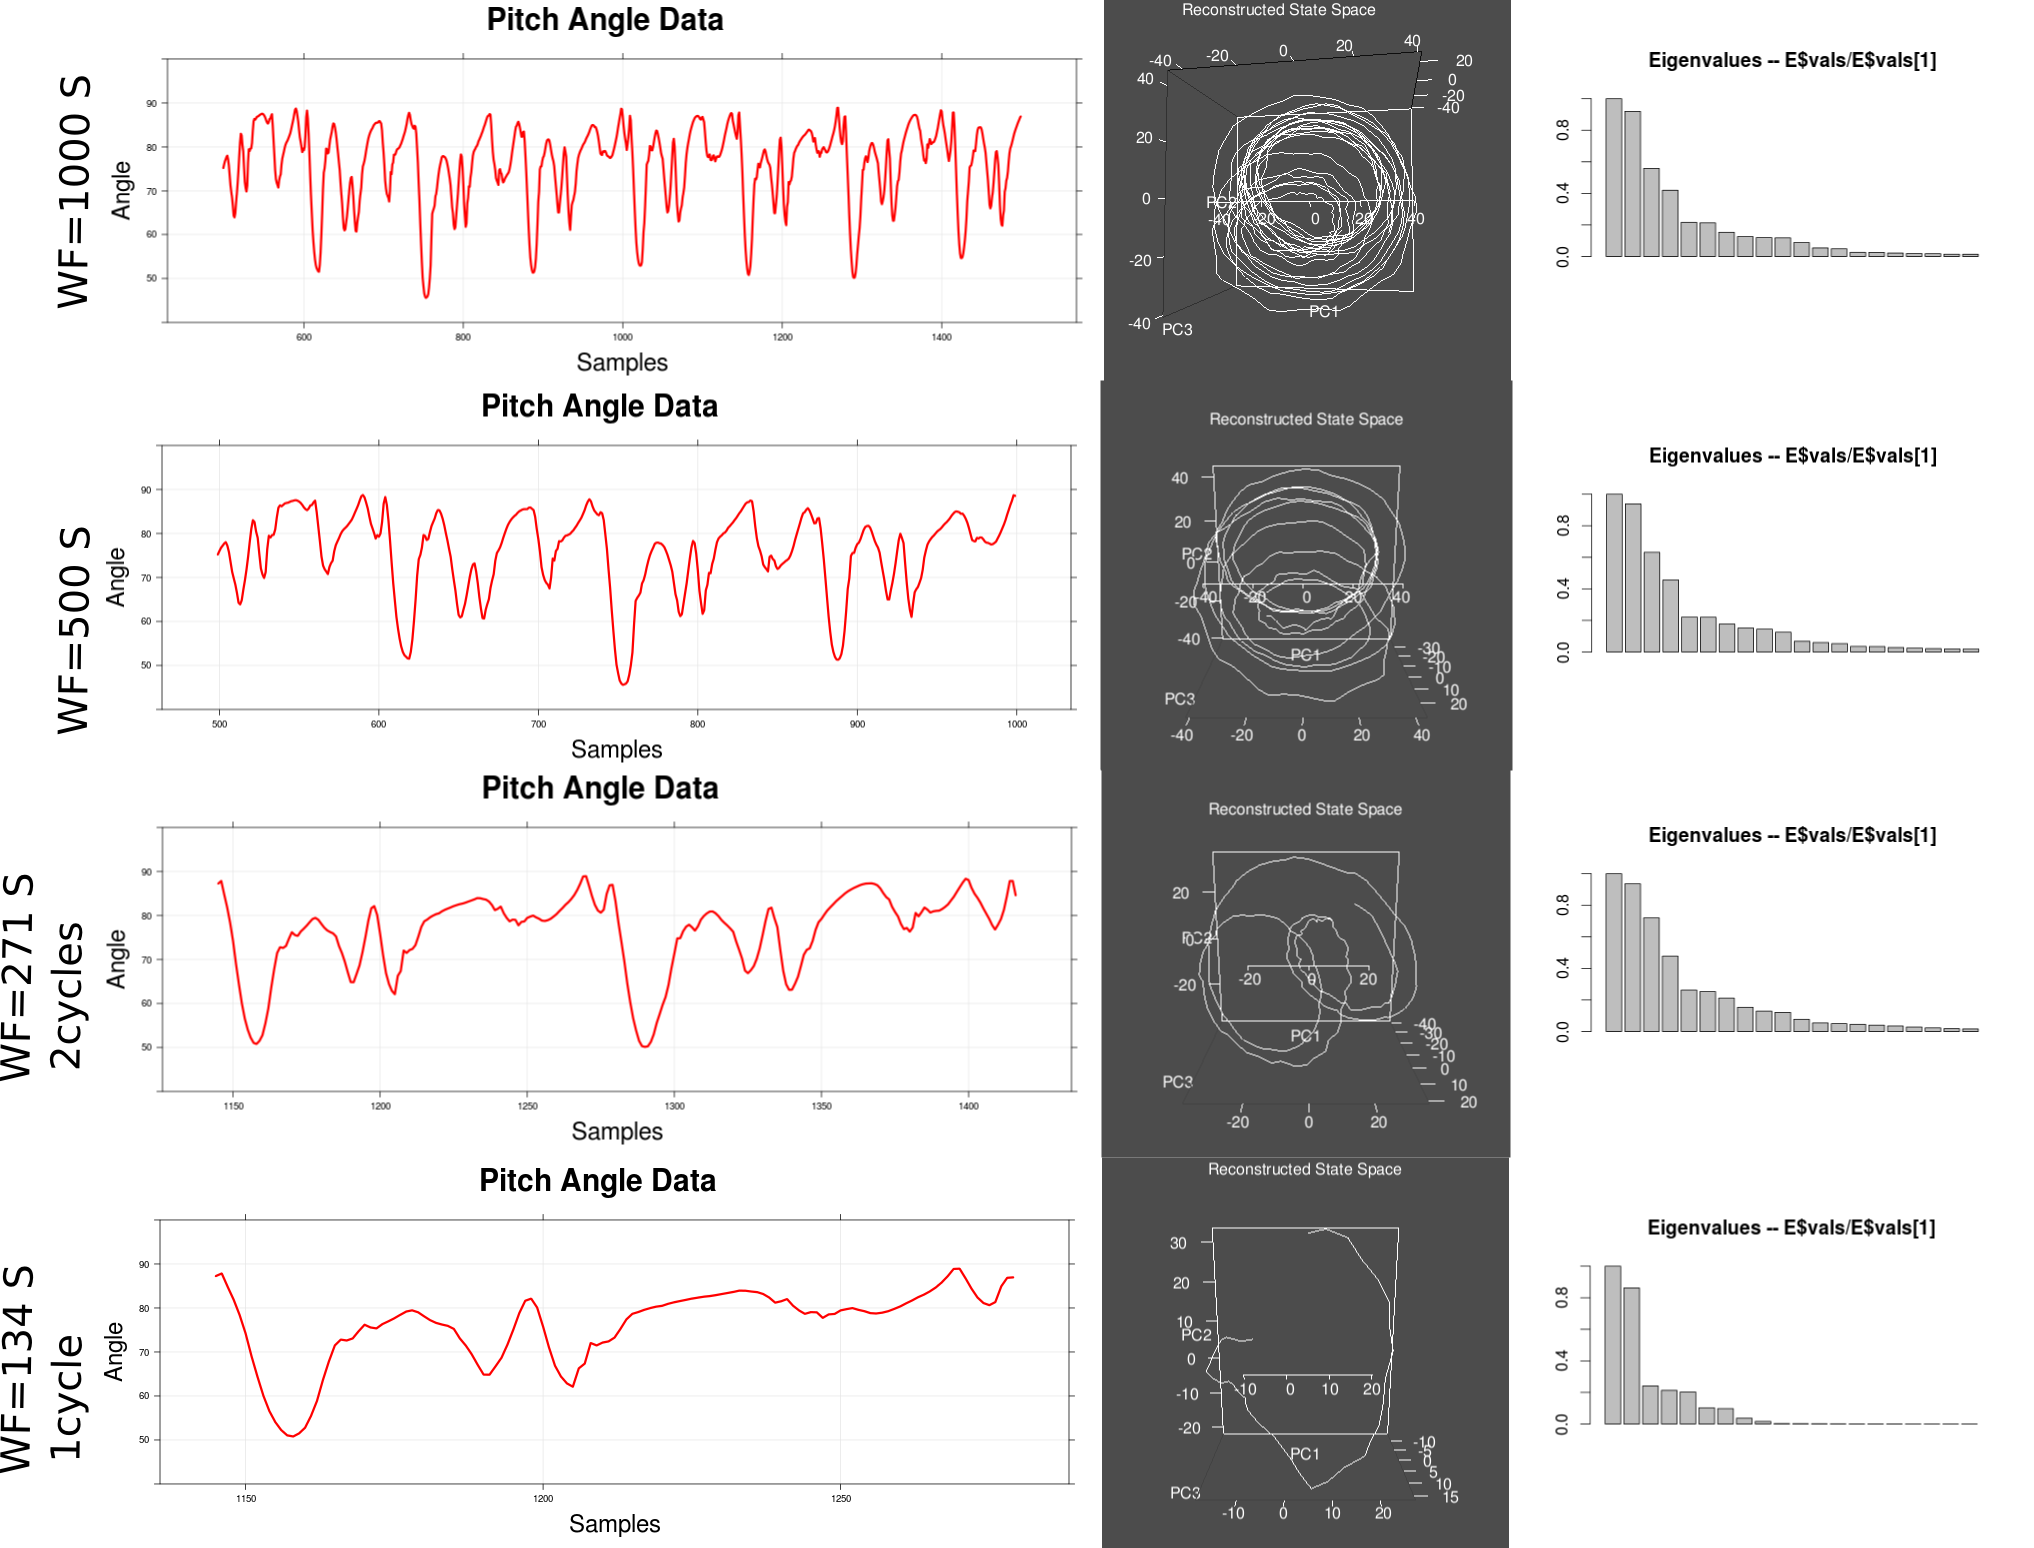
\includegraphics[scale=0.129]{cumbia}
\caption{3D Reconstructed State Space and Eigenvalues}
\end{figure}  
\end{frame}
%---------------------------------------------------


%+++++++++++++++++++++++++++++++++++++++++++++++++++
\begin{frame}
\frametitle{Pitch Angle Time Series for Salsa}

\begin{figure}
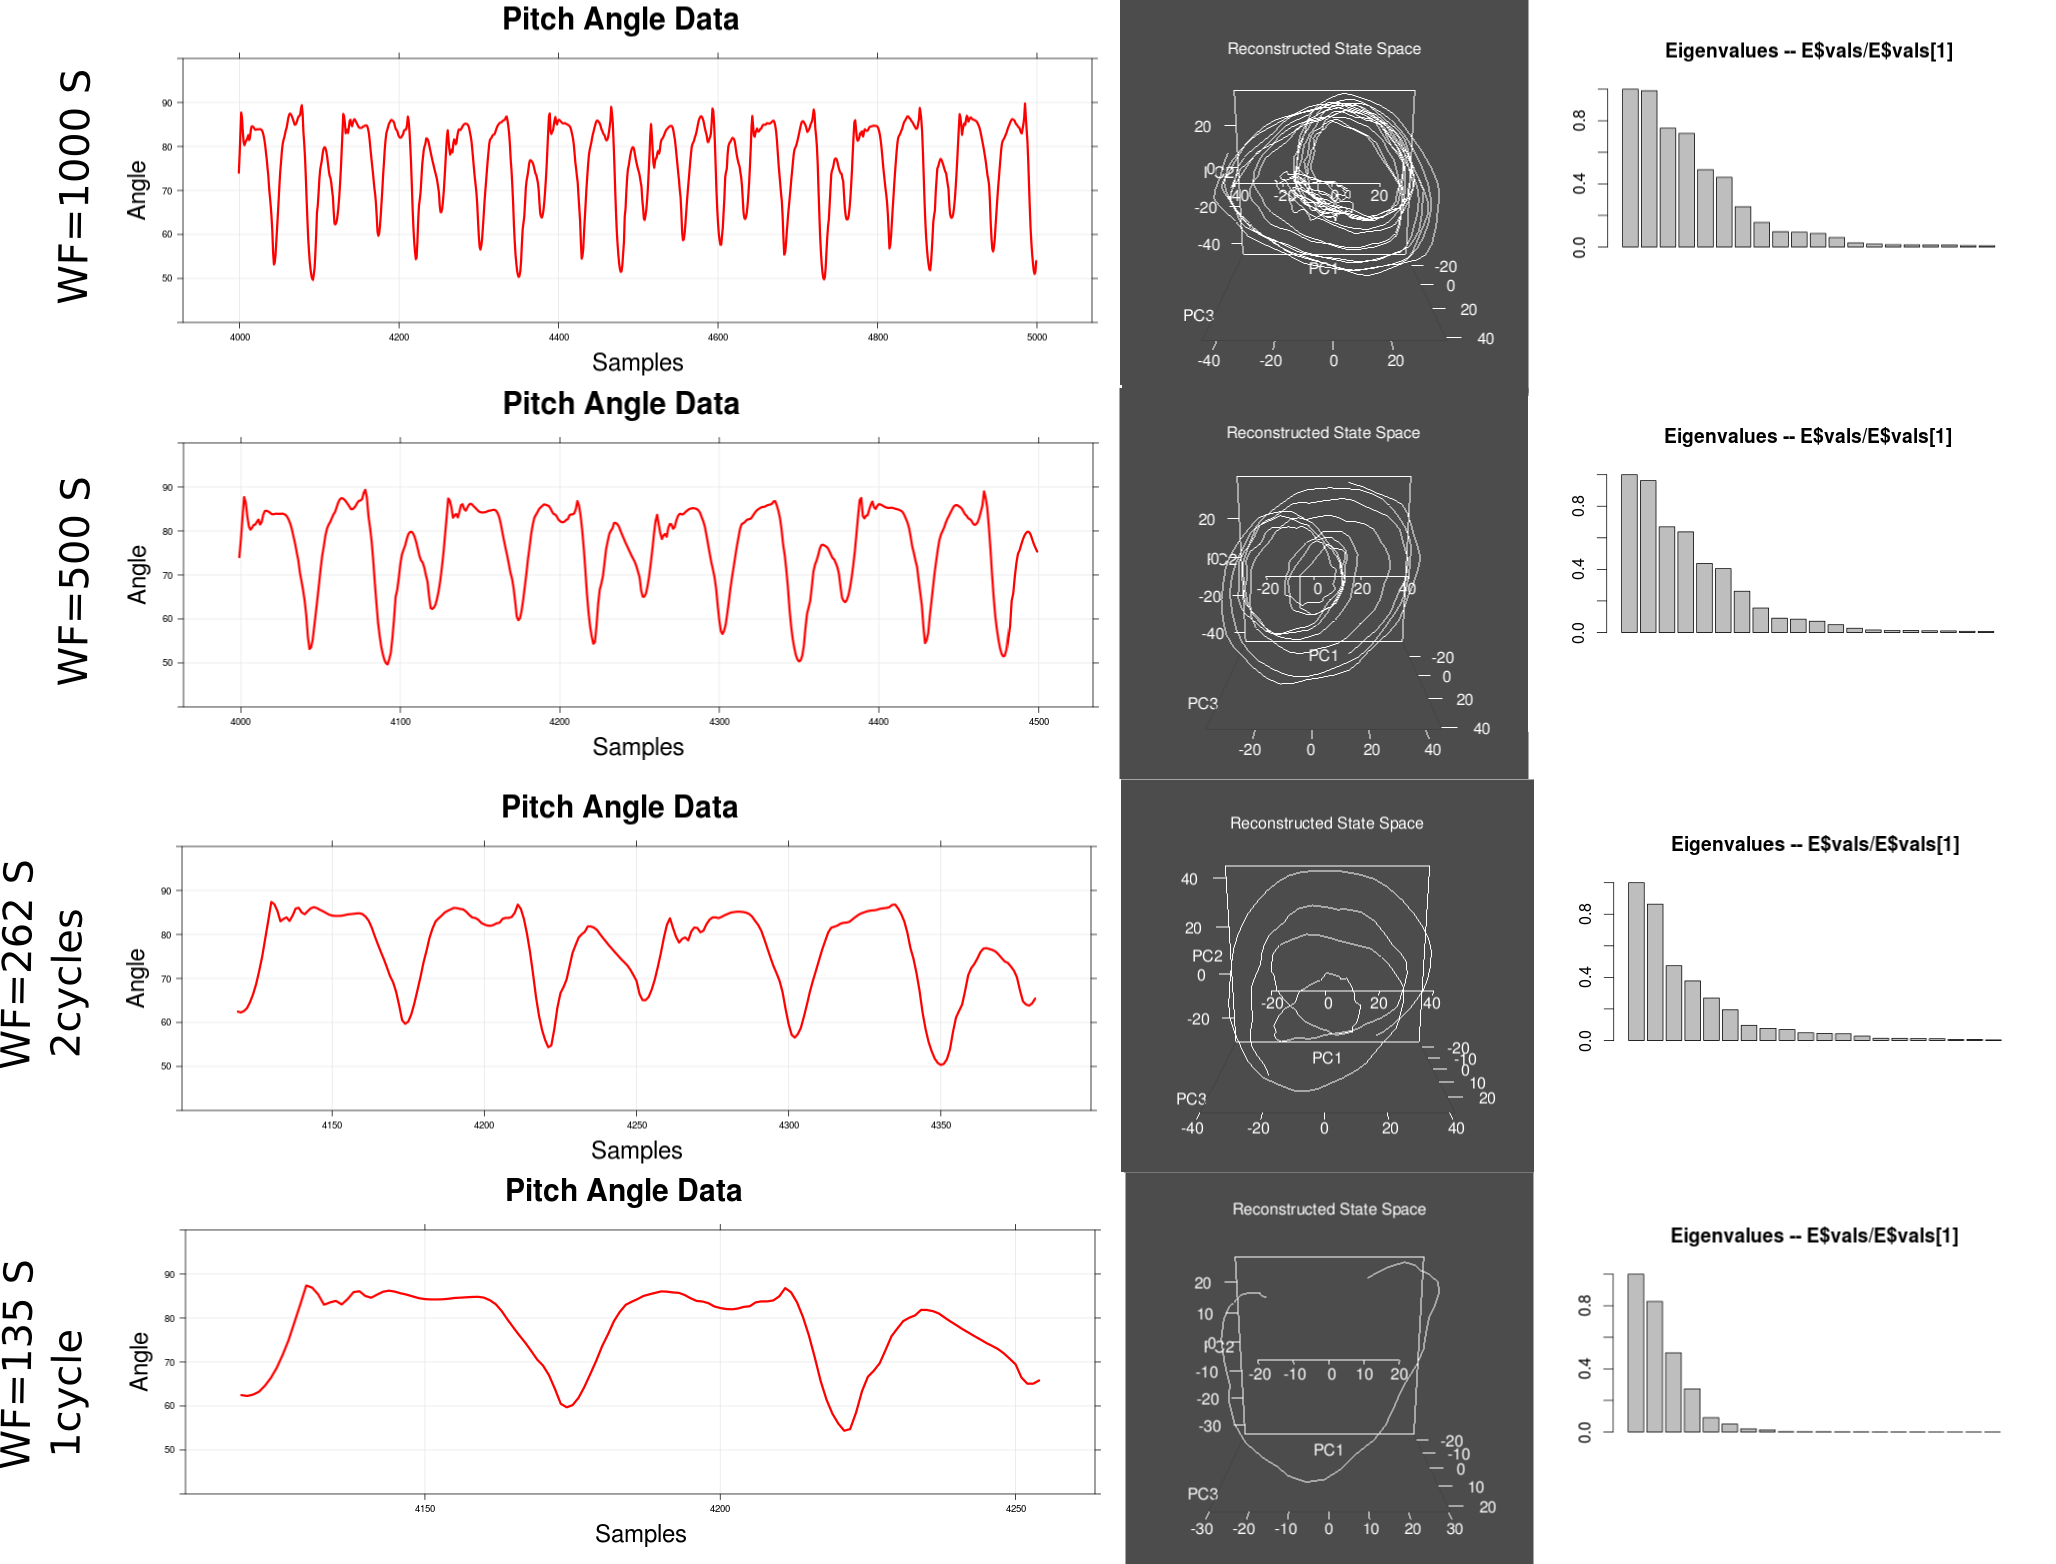
\includegraphics[scale=0.129]{salsa}
\caption{3D Reconstructed State Space and Eigenvalues}
\end{figure}  
\end{frame}
%---------------------------------------------------



\section{Challenges for the PhD research}


%+++++++++++++++++++++++++++++++++++++++++++++++++++
\begin{frame}
\frametitle{??????????????????????}

TECHNICAL CHALLENGES
 \begin{itemize}
 \item Build a body sensor network and determine how many sensors and 
 where are the optimal places to wear this sensors [Mannini et al. 2013].
 \item Create its c++ library as a open source software for the human motion capture system
 \item Implement machine learning algorithms and evaluate the human activity recognition in a real-time performance.
\end{itemize}

RESEARCHABLE CHALLENGES
  \begin{itemize}
   \item Which non-reported concepts from nonlinear dynamics 
  can be used to obtain features in the human body analysis?
  \item Does the use of concepts from nonlinear dynamics 
  using Inertial Measurement Units can recognise up to 50 human
  activities as reported in [Reddy et al. 2012]?
  \end{itemize}

\end{frame}
%---------------------------------------------------

%+++++++++++++++++++++++++++++++++++++++++++++++++++
\begin{frame}
\frametitle{}

\vspace{2cm}
\begin{center}
\LARGE{QUESTIONS?} 
\end{center}

\vspace{1cm}

\normalsize 
\textbf{P\'erez-Xochicale Miguel Angel} \\

E-Mail: {\color{blue} \href{mailto:MAP479@bham.ac.uk}{MAP479@bham.ac.uk} } 

Homepage:
{\color{blue} \href{https://sites.google.com/site/perezxochicale/}{https://sites.google.com/site/perezxochicale/} }
\vspace{1cm}



\includegraphics[scale=.4]{CC4}
\tiny{ 
\textbf{My own pictures are release under CC BY-NC 4.0
{\color{blue} \href{http://creativecommons.org/licenses/by-nc/4.0/}{http://creativecommons.org/licenses/by-nc/4.0/} } \\
Give credits to: P\'erez Xochicale M. A.
}
}







\end{frame}
%---------------------------------------------------




\end{document}

